\documentclass[a4paper,twoside,english]{report}
\usepackage[utf8]{inputenc}
\setcounter{secnumdepth}{3}
\usepackage{babel}
\usepackage{array}
\usepackage{booktabs}
\usepackage{textcomp}
\usepackage{url}
\usepackage{multirow}
\usepackage{amsmath}
\usepackage{graphicx}
\usepackage[authoryear]{natbib}
\usepackage{nomencl}
\providecommand{\printnomenclature}{\printglossary}
\providecommand{\makenomenclature}{\makeglossary}
\makenomenclature
\usepackage[unicode=true,
 bookmarks=false,
 breaklinks=false,pdfborder={0 0 1},backref=section,colorlinks=false]
 {hyperref}
\usepackage{breakurl}
\usepackage{etoolbox}
\makeatletter
\patchcmd{\Ginclude@eps}{"#1"}{#1}{}{}
\makeatother

\makeatletter
\special{papersize=\the\paperwidth,\the\paperheight}

\newcommand{\noun}[1]{\textsc{#1}}
\providecommand{\tabularnewline}{\\}
\newcommand{\lyxdot}{.}


\usepackage[colorinlistoftodos]{todonotes}
\usepackage{placeins}
\usepackage{parskip}



\usepackage{subcaption}
\usepackage{tikz}

\usepackage{array}

\usepackage{amssymb}


\usepackage{graphicx}

\usepackage{booktabs}
\newcommand{\otoprule}{\midrule[\heavyrulewidth]}

\usepackage{pdflscape}
\usepackage{bbding}
\usepackage{pifont}

\makeatother

\begin{document}
\thispagestyle{empty}

\vspace*{3cm}

\begin{center}
{\LARGE{}Marine cybernetics}
\par\end{center}{\LARGE \par}

\begin{center}
{\LARGE{}laboratory handbook }
\par\end{center}{\LARGE \par}

\begin{flushleft}
\vfill{}
\par\end{flushleft}

\begin{flushleft}

\includegraphics[scale=0.6]{fig/NTNU_logo}
\par\end{flushleft}

Faculty of Engineering Science and Technology\\
Department of Marine Technology

\clearpage{}\thispagestyle{empty}\vspace*{3cm}

\clearpage{}

\pagenumbering{roman}\setcounter{page}{1}

\vspace*{3cm}


\section*{Introduction}

This handbook is a comprehensive reference for the marine cybernetics
laboratory. The laboratory is used in teaching and research on development
and real-time testing of marine control systems.

\section*{Structure}

Part \ref{part: Theory} explains the concepts and motivations for
the stepwise controller development.

Part \ref{part: Laboratory user guide} is a user guide intended for
users of the laboratory. Step-by-step instructions for development
and deployment of programs to the real-time controller are given.

Lower level details, intended for laboratory assistants and customized
use, are given in Part \ref{part: Equipment setup and configuration}.

\newpage{}\tableofcontents{}

\newpage{}\settowidth{\nomlabelwidth}{MC Lab}
\printnomenclature{}

\nomenclature{BT}{bow thruster}

\nomenclature{cRIO}{compact reconfigurable input/output real-time embedded industrial controller by National Instruments}

\nomenclature{CS}{cybership ship prefix}

\nomenclature{CSE1}{CS Enterprise I}

\nomenclature{CSS}{CS Saucer}

\nomenclature{DP}{dynamic positioning}

\nomenclature{ESC}{electronic speed controller}

\nomenclature{FPGA}{field-programmable gate array}

\nomenclature{HIL}{hardware-in-the-loop}

\nomenclature{IO}{input/output}

\nomenclature{MC Lab}{marine cybernetics laboratory}

\nomenclature{PWM}{pulse-width modulation}

\nomenclature{RPi}{Raspberry Pi single-board computer}

\nomenclature{VSP}{Voith Schneider propeller}

\newpage{}

\pagenumbering{arabic}

\part{Introduction}\label{part: Theory}

\chapter{Marine cybernetics laboratory}

\begin{figure}
\centering 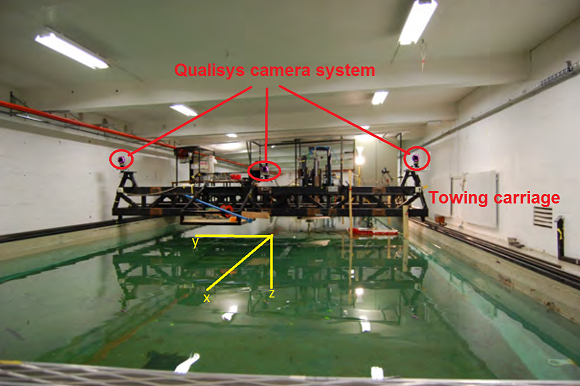
\includegraphics[width=0.95\textwidth]{fig/mc_lab} 
\caption{Marine cybernetics laboratory basin}
\label{fig: Marine cybernetics laboratory basin-1}
\end{figure}

The laboratory is equipped for experimental testing of marine control
systems and hydrodynamic tests. It consists of a wave basin with an
advanced instrumentation package and a towing carriage. The basin,
depicted in Figure \ref{fig: Marine cybernetics laboratory basin-1},
has dimensions 40m x 6.45m x 1.5m (LxBxD).

The laboratory gives tangible results that solidifies theoretical
work. 
\clearpage{}

\section{Fixed Equipment}

\subsection{Qualisys motion capture system}
Qualisys provides 6 degrees of freedom data tracking. The system has millimeter precision, works in real time and is configured to 50Hz.

The positioning system consists of three Oqus high speed infrared cameras registering infrared reflectors placed on the vessel. Peer-to-peer (P2P) networking is used to transmit camera data to a dedicated computer running Qualisys Track Manager (QTM) software. QTM performs triangulation and broadcasts the vessel position over the wireless network.

\subsection{Towing carriage}

The carriage runs at speeds up to 2m/s. It also has capability for
precise movement of models in 6 degrees of freedom and is thus suitable
for more specialized hydrodynamic tests.

\subsection{Wave generator}

\begin{table}
\centering{}%
\begin{tabular}{lll}
\hline 
 & Height {[}m{]} & Period T {[}s{]}\tabularnewline
\hline 
Regular waves & $H<0.25$ & 0.3 - 3.0\tabularnewline
Irregular waves & \textbf{$H_{s}<0.15$} & 0.6 - 1.5\tabularnewline
\hline 
\end{tabular}\caption{\label{tab:Wave generator capacity-1}Wave generator capacity}
\end{table}

The single paddle wave generator is controlled by a dedicated computer.
Available spectrum are first order Stoke, JONSWAP, Pierson-Moskowitz,
Bretschneider, ISSC and ITTC. Table \ref{tab:Wave generator capacity-1}
summarizes the generation capacity.

\subsection{Current generator}

Not available as of spring 2015.

\clearpage{}

\section{Vessels}

Several both surface and underwater vessels are used in the MC Lab.

The cyber ship class, with ship prefix CS, consists of 6 vessels:
\begin{itemize}
\item CS Inocean Cat I Arctic Drillship,
\item CS Saucer,
\item CS Enterprise I,
\item Cybership III,
\item Cybership II, and
\item Cybership I.
\end{itemize}
Also, there laboratory holds an underwater craft,
\begin{itemize}
\item ROV Neptunus,
\end{itemize}
and a semi submersible drilling rig
\begin{itemize}
\item CyberRig.
\end{itemize}
\clearpage{}

\subsection{CS Inocean Cat I Arctic Drillship}

\todo{Add material from Jon}

\clearpage{}

\subsection{CS Saucer}

\begin{figure}
\centering 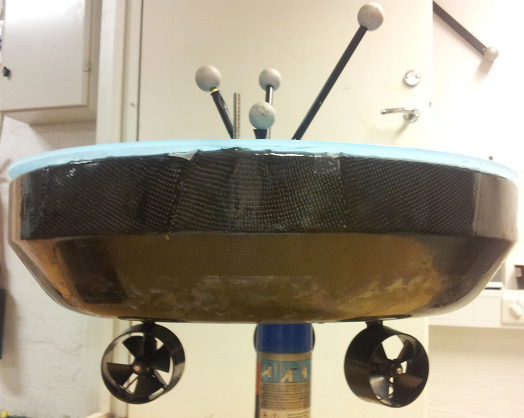
\includegraphics[width=0.95\textwidth]{fig/CSSaucer} 
\caption{CS Saucer}
\label{fig: CS Saucer}
\end{figure}

CS Saucer is a fully actuated and highly controllable vessel with
a spherically shaped hull, much like a flying saucer. It is designed
to be light weight, agile and very responsive. The CS Saucer adds
possibilities for rapid response and motion in surge and sway, something
that is difficult to obtain with a traditional ship hull. 

The non conventional shape of the hull of such a marine vessel opens
the possibilities for original projects in control theory and hydrodynamics,
as well as serving as a platform where student can get experience
with the practical aspects of control systems implementation

\subsubsection{Hull}

The hull is constructed from three millimeter MDF sheeting, milled
Divinycell foam and a woven carbon with epoxy. This results in a rigid
hull with low draft. The vessel has a detachable lid made of Plexiglas
which is secured to the top of the vessel with four butterfly screws.

\subsubsection{Control system}

The embedded controller myRIO from National Instruments is used to
control the vessel. The myRIO with its default FPGA personality is
capable of driving 8 PWM signals simultaneously, in addition to multiple
digital and analog connections. 

Marine 30 Electronic Speed Controllers (ESC) are used to control the
DC motors driving the thruster propellers.

\subsubsection{Actuators}

The vessel is fitted with three Graupner Schottel drive unit II azimuth
thrusters. Torpedo 800 brushed DC motors drive the propeller. Graupner
DS8311 servo motors are used to control the angle of the thrusters.

\subsubsection{Power}

\begin{figure}
\centering 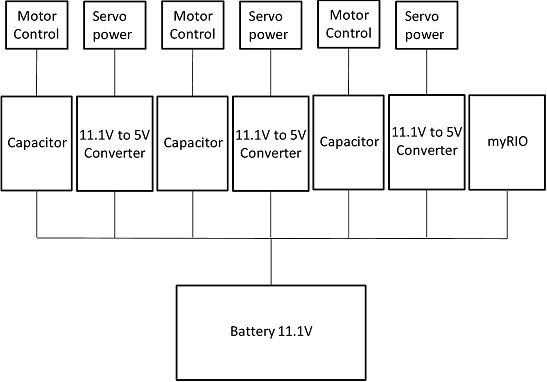
\includegraphics[width=0.95\textwidth]{fig/CSSaucer_power}
\caption{\label{fig: CS Saucer power}CS Saucer power system}
\end{figure}

The system is powered by a three cell 11.1V Lithium Polymer battery,
as seen in Figure \ref{fig: CS Saucer power}

In order to convert the 11.1V power provided by the battery to 5V
for the servos, a switching DC/DC converter is user together with
a capacitor.

\subsubsection{Literature}

\paragraph{Specialization projects and master theses}
\begin{itemize}
\item Marine Cybernetics Vessel CS Saucer: Design, construction and control
\citep{Idland2015} 
\item Rotem Sharoni, 2016
\item Einar Skiftestad Ueland, 2016
\end{itemize}
\clearpage{}

\subsection{ROV Neptunus}

\begin{figure}
\centering 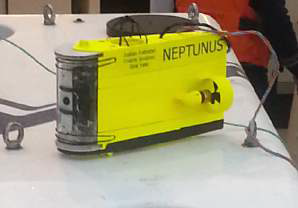
\includegraphics[width=0.4\textwidth]{fig/ROVNeptunus_1}
\caption{\label{fig: ROV Neptunus}ROV Neptunus}
\end{figure}

Neptunus is a small, low-cost ROV prototype. The design is based on
OpenROV, and the instrumentation is directly adapted thence.

\subsubsection{Hull}

Neptunus is designed with a foil shaped body, in order to induce low
drag forces in the longitudinal direction. The prototype consists
of several blocks, made of acrylonitrile butadiene styrene (ABS) -
plastic, 3D printed at NTNU.

\subsubsection{Actuators}

There are three thrusters on Neptunus: two in the longitudinal direction,
and one in the vertical.

\subsubsection{Control system}

The main processes are driven by a BeagleBone computer, and an Arduino
control board. It is equipped with an inertial measurement unit (IMU)
and a high definition (HD) web camera.

\subsubsection{Literature}

\paragraph{Specialization projects and master theses}
\begin{itemize}
\item Low cost ROV design, based on testing, simulations and analysis of
OpenROV\citep{FollestadSandvedValle2014}
\item Design and Implementation of Software for the ROV Neptunus \citep{Munz2015}
\item Remote Control and Automatic Path-following for C/S Enterprise I and
ROV Neptunus \citep{Sandved2015}
\end{itemize}
\clearpage{}

\subsection{CS Enterprise I}

\begin{figure}
\centering 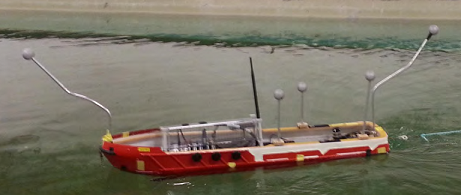
\includegraphics[width=0.95\textwidth]{fig/CSE1_2} \caption{\label{fig: Cybership Enterprise 1}CS Enterprise I}
\end{figure}

The CSE1, depicted in Figure \ref{fig: Cybership Enterprise 1}, \todo{hva
bruker vi den til}

The vessel CS Enterprise I was constructed as a model ship available
to master and PhD students at NTNU {[}Skatun, 2011{]}. The work performed
on CS Enterprise I include, but is not limited to, dynamic positioning
systems, maneuvering systems and path following, and navigation with
virtual reality {[}Valle, 2015{]}.

\subsubsection{Hull}

tug boat model.

\subsubsection{Actuators}

The ship is fitted with two Voith Schneider propellers (VSP) astern
and a bow thruster (BT).

\subsubsection{Control system}

The on-board control system consists of
\begin{itemize}
\item a National Instruments compact reconfigurable input/output (cRIO)
embedded controller,
\item a Raspberry Pi (RPi) single-board computer,
\item three electronic speed controllers (ESC), and
\item four servos.
\end{itemize}
The operator interfaces the system by
\begin{itemize}
\item laptop, and
\item a Sony Sixaxis wireless gamepad for PlayStation 3.
\end{itemize}

\paragraph{High-level communication}

\begin{figure}
\begin{centering}
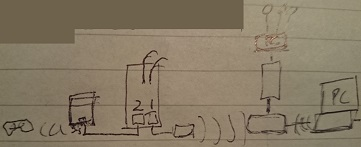
\includegraphics[width=0.8\textwidth]{fig/setupCSE1}
\par\end{centering}
\caption{\label{fig: CSE1 communication}CSE1 communication diagram}

\end{figure}

\begin{figure}
\begin{centering}
\includegraphics[height=0.4\paperheight]{fig/"CSE1 signal".png}
\par\end{centering}
\caption{\label{fig: CSE1 signal}CSE1 signal paths}
\end{figure}

Following Figure \ref{fig: CSE1 communication} from left to right:
\begin{description}
\item [{Sixaxis}] transmits its information to the RPi Bluetooth USB dongle
with which it is previously paired\footnote{One-time pairing procedure described in Appendix \ref{par: Bluetooth-pairing}.}.
\item [{RPi}] receives Sixaxis data through the USB dongle and forwards
it through its TCP/IP\footnote{All IP addresses are as given in Table \ref{tab: IP addresses}.}
server over Ethernet to the cRIO.
\item [{cRIO}] reads QTM broadcast positioning data through the Wi-Fi bridge
on Ethernet port 1, Sixaxis data on Ethernet port 2. Online data and
laptop input is transmitted and received on Ethernet port 1 by the
VeriStand Engine.
\item [{Laptop}] reads simulation data and sends input to the cRIO over
Ethernet.
\end{description}

\paragraph{Low-level communication}

The BT and VSP motor speeds are controlled by ESC. The ESC receive
their setpoints as a pulse-width modulated (PWM) signals from the
cRIO digital output module.

The VSP blade pitches are controlled by servos. The servos also receive
their setpoint as PWM signals.

\paragraph{Software}

\begin{figure}
\begin{centering}
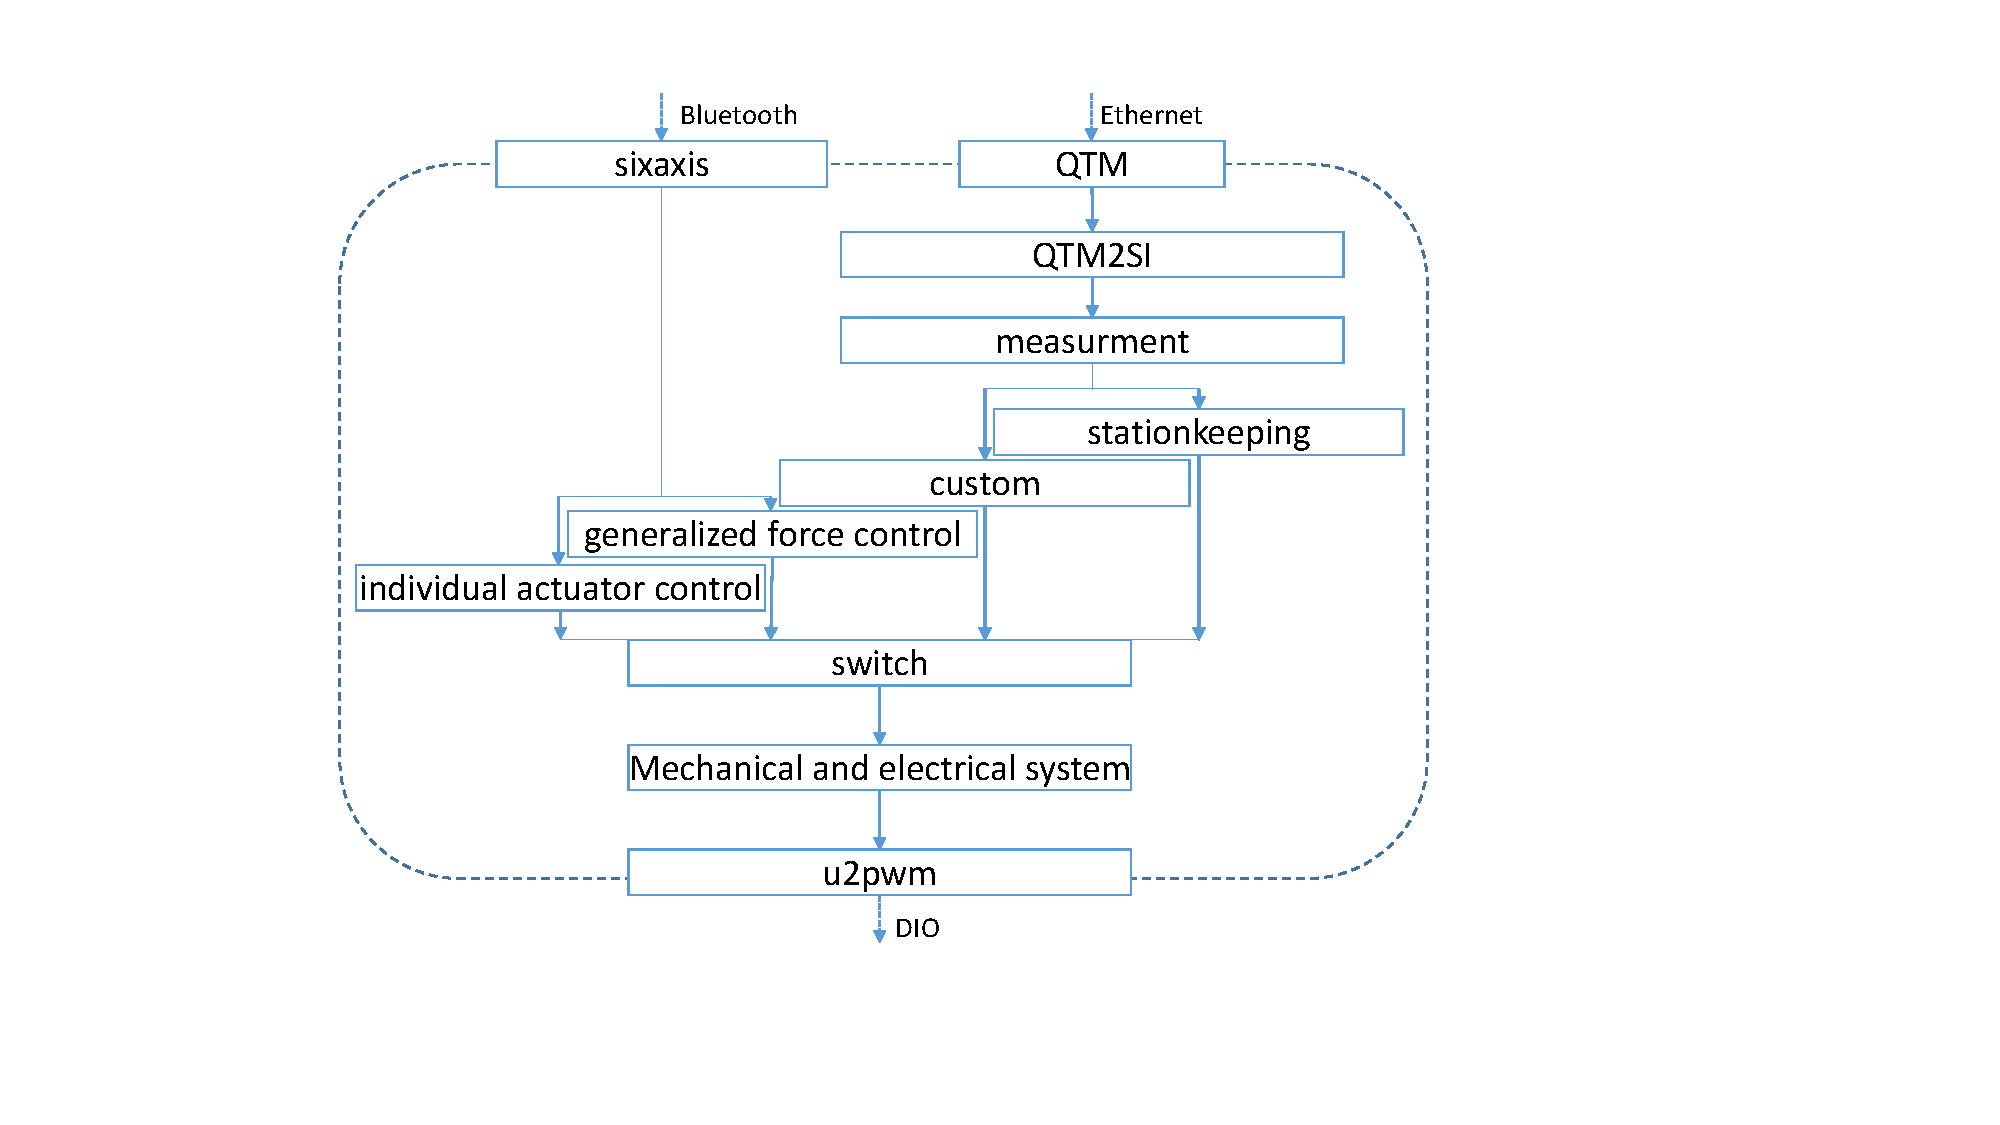
\includegraphics[height=0.6\textwidth]{fig/CSE1_ctrl_software.pdf}
\par\end{centering}
\caption{\label{fig: CSE1 software}CSE1 control software}
\end{figure}

The software supports four different control modes, as seen in the
middle of Figure \ref{fig: CSE1 software}:
\begin{itemize}
\item Individual actuator control allows controlling the force $u$, angular
velocity $\omega$ and angle $\alpha$ each thruster
\item Generalized force control facilitates inputting desired surge and
sway forces and yaw moment, $X$, $Y$, $N$, respectively.
\item The user defined custom control
\item Stationkeeping.
\end{itemize}
The two first modes only take the joystick signal as input.

The two latter modes take the position measurement $\eta_{\text{QTM}}$
from QTM. This signal is in turn converted meters and radians. Finally,
measurement noise may be added to get the measured signal $\eta_{m}$.

The control modes output the desired output vector $u_{d}$. The actual
output $u$ may differ due to mechanical and electrical dynamics.

Finally, the output is converted to pwm signals outputted through
the digital input/output (DIO) port.

\subsubsection{Power}

\begin{figure}
\begin{centering}
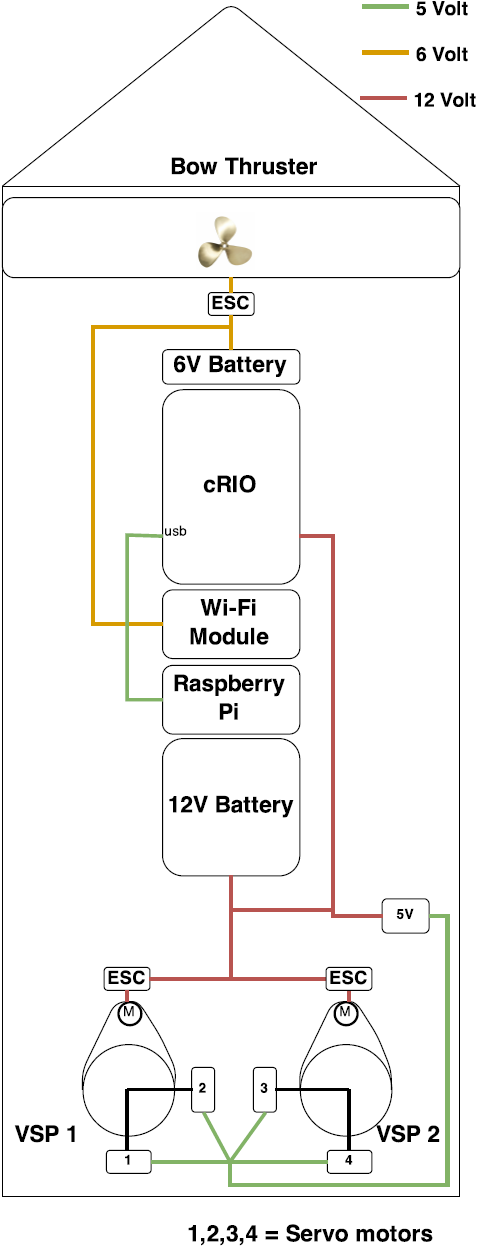
\includegraphics[height=0.4\paperheight]{fig/CSE1_power}
\par\end{centering}
\caption{\label{fig: CSE1 power}CSE1 power system}
\end{figure}

See Figure \ref{fig: CSE1 power}.

\subsubsection{Literature}

\paragraph{Journals and conferences}
\begin{itemize}
\item LOS guidance for towing an iceberg along a straight-line path \citep{OrstenNorgrenSkjetne2014}
\end{itemize}

\paragraph{Specialization projects and master theses}
\begin{itemize}
\item Development of a DP system for CS Enterprise I with Voith Schneider
thrusters. \citep{Skaatun2011}
\item Development of a modularized control architecture for CS Enterprise
I for path-following based on LOS and maneuvering theory \citep{Tran2013}
\item Automatic Reliability-based Control of Iceberg Towing in Open Waters
\citep{Orsten2014}
\item Line-Of-Sight-based maneuvering control design, implementation, and
experimental testing for the model ship C/S Enterprise I.\citep{Tran2014}
\item Remote Control and Automatic Path-following for C/S Enterprise I and
ROV Neptunus \citep{Sandved2015}
\item Marine Telepresence System \citep{Valle2015}
\item Elias Bjørne, 2016
\end{itemize}

\paragraph{Other}
\begin{itemize}
\item YouTube video \citep{Skaatun2014}
\end{itemize}

\subsubsection{Further development}
\begin{itemize}
\item Implement “fail to zero” for communication breakdown
\item Add IMU or gyro
\end{itemize}
\clearpage{}

\subsection{Cybership III}

1:30 scale model of a supply vessel.

\clearpage{}

\subsection{Cybership II}

2001. 1:70 scaled model of a supply vessel.\clearpage{}

\subsection{Cybership I}

1:70 scaled model of a supply vessel.

\clearpage{}

\subsection{CyberRig}

The CyberRig is a semi submersible 1:100 scaled model drilling rig
used in student projects and research {[}Bjrneset, 2014{]}.

\clearpage{}

\subsection{Our Lass II model}

\begin{figure}
\centering 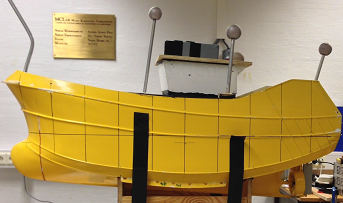
\includegraphics[width=0.95\textwidth]{fig/ourlass} \caption{\label{fig: Our Lass II}Our Lass II}
\end{figure}

1:24 scaled model of a fishing vessel

\subsubsection{Literature}

\paragraph{Journals and conferences}
\begin{itemize}
\item Online Estimation of Ship’s Mass and Center of Mass Using Inertial
Measurements \citep{LinderEnqvistFossenJohansenGustafsson2015}
\end{itemize}
\clearpage{}

\chapter{Control system development philosophy}

As the complexity of marine vessels and operations grows, the need
for thorough testing and verification of the vessel real-time control
and monitoring systems increases. More advanced integrated functionality
relies on many separately designed control and monitoring systems
to cooperate on performing common tasks. Regular software simulations
cannot cover all aspects of this complexity.

Through steps-wise verification and validation at different levels
of fidelity, errors can be discovered at earlier stages thus lowering
the total development cost.

In the case of the MC Lab, users qualify their experimental setups
before the assigned laboratory time. This reduces debugging time,
improves tuning of parameters and test scenarios, thereby increasing
efficiency and maximizing the outcome of the experimental work.

\clearpage{}

\section{Development Steps}

Marine cybernetics deals with control engineering for the vessel mechatronic
systems which again interact with the environment. In this section,
``the controller'' refers to the designed control software and ``the
plant'' to the combination of the mechatronic system and the environment.

\subsection{Model-in-the-Loop}

\subsubsection{Principle}

A model of the controller interconnected with a physical model of
the plant, in a control development environment, such as MATLAB Simulink.

\subsubsection{Aim}

Develop control strategies . Test principles.

\subsubsection{Iteration time}

Extremely short, small changes are immediately implemented and tested.

\subsubsection{Cost}

Low

\subsection{Software-in-the-Loop}

The controller is coded in the final language, such as C or C++, and
connected to the plant model in a control development environment.

\subsubsection{Aim}

Test of coding system. Reveal coding failures.

\subsubsection{Iteration time}

Slightly longer than MIL.

\subsection{Processor-in-the-Loop}

\subsubsection{Principle}

The controller is deployed to a representative microprocessor, connected
to the plant simulation via high speed bus, such as JTAG. The plant
must be synchronized with the controller.

\subsubsection{Aim}

Expose problems with execution in the embedded environment, such as
insufficient computing resources on the embedded processor.

\subsubsection{Iteration time}

Higher, due to the need to regenerate and deploy code for each run.

\subsection{Hardware-in-the-Loop}

\subsubsection{Principle}

Controller fully installed into the intended final hardware, connected
through the plant only through the proper IO. The plant simulator
must run on a real-time computer emulating the IO of a real process.

\subsubsection{Aim}

Perform regulation, security and failure tests without risk.

Investigate the interaction between subsystems.

Ensure a high level of robustness and quality.

\subsection{Scale test}

-

\subsection{Full scale}

-

\clearpage{}

\section{Recommended Control Modes}

It is favorable to allow for five main control modes:
\begin{itemize}
\item Stop all actuators
\end{itemize}
\begin{enumerate}
\item Individual actuator control
\item Generalized force control
\item Regulation
\item Operations
\end{enumerate}
In addition, sub-modes may allow more functionality. 

\subsection{Individual actuator control}

\begin{figure}
\centering 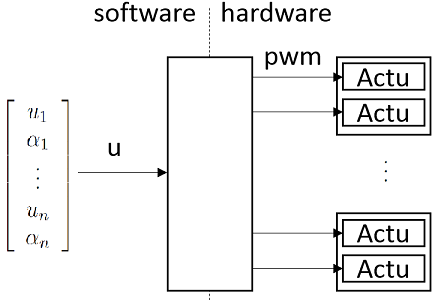
\includegraphics[scale=0.45]{fig/ctrl_u} \caption{\label{fig: Individual actuator control}Individual actuator control}
\end{figure}

The most basic mode allows controlling each thruster separately. Inputs
are typically normalized force $u=\left[-1,1\right]$, angle $\alpha=\left[-\pi,\pi\right]$,
and sometimes normalized rotational speed $\omega=\left[-1,1\right]$.
The software computes the corresponding physical signal, for instance
a pulse width manipulated (PWM) signal as illustrated in Figure \ref{fig: Individual actuator control}.

The user interface may be through gamepad, computer, tablet, etc.

Implementation details are discussed in Appendix \ref{subsec:Direct-Thruster-Control}.

\subsection{Generalized force control}

\begin{figure}
\centering 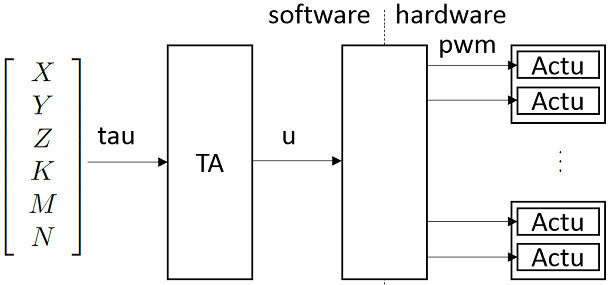
\includegraphics[scale=0.45]{fig/ctrl_tau} \caption{\label{fig: Generalized force control}Generalized force control}
\end{figure}

Thrust allocation allows input of the desired generalized force, as
seen in Figure \ref{fig: Generalized force control}. For six degrees
of freedom (6 DOF) control the input is 
\[
\tau=\left[\begin{array}{c}
X\\
Y\\
Z\\
K\\
M\\
N
\end{array}\right].
\]
For surface craft, 3 DOF are typically considered: 
\[
\tau=\left[\begin{array}{c}
X\\
Y\\
N
\end{array}\right].
\]

The user interface may be through gamepad, computer, tablet, etc.
The appropriate reference frame depends on the application.

\subsubsection{Body frame}

Most commonly, the desired thrust is given in the vessel-fixed body
frame. This is the intuitive setup for an on-board operator.

Implementation details are discussed in Appendix \ref{subsec:Direct-Body-relative-motion}.

\subsubsection{Inertial frame}

For remote operation, it may be suitable to input the force with regard
to the inertial frame, rather than the vessel orientation.

Implementation details are discussed in Appendix \ref{subsec:Direct-NED-relative-motion}.

\subsubsection{User frame}

When the operator has eye contact with the vessel, it may be suitable
to specify the force with respect to the line of sight between the
operator and craft. 

Implementation details are discussed in Appendix \ref{subsec:Direct-User-relative-motion}.

\subsection{Regulation}

\begin{figure}
\centering 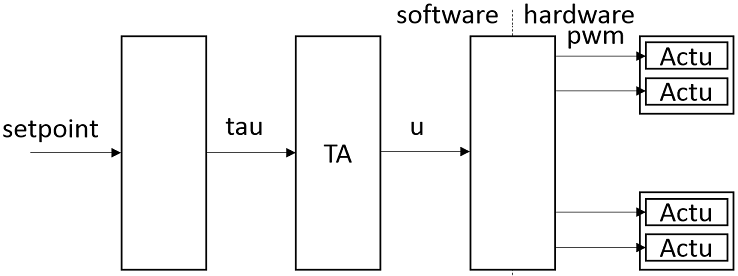
\includegraphics[scale=0.45]{fig/ctrl_setpoint} \caption{\label{fig: Regulation}Regulation}
\end{figure}

\begin{table}
\begin{centering}
\begin{tabular}{lcccccc}
 & $x$ & $y$  & $z$ & $\phi$ & $\theta$ & $\psi$\tabularnewline
\hline 
Stationkeeping & \ding{51} & \ding{51} &  &  &  & \ding{51}\tabularnewline
Heading &  &  &  & \ding{51} &  & \tabularnewline
Depth &  &  & \ding{51} &  &  & \tabularnewline
Roll/Pitch &  &  &  & \ding{51} & \ding{51} & \tabularnewline
\end{tabular}
\par\end{centering}
\caption{\label{tab:Regulation-modes}A selection of regulation modes}
\end{table}

Maintaining a given value in one or several DOFs under the influence
of disturbances is the basic automatic control mode. The given value
is called setpoint, as illustrated in Figure \ref{fig: Regulation}.
Typical sub-modes are listed in Table \ref{tab:Regulation-modes}.
Reference filters for changing setpoints may or may not be included.

The user interface typically allows inputting the setpoint value directly,
for instance on a computer or tablet. Alternatively, the setpoint
may be translated through gamepad.

Further details are discussed in Appendix \ref{subsec:Auto-Control}.

\subsection{\label{subsec:Marine-Operations-Control-1}Marine Operations Control}

\begin{figure}
\centering 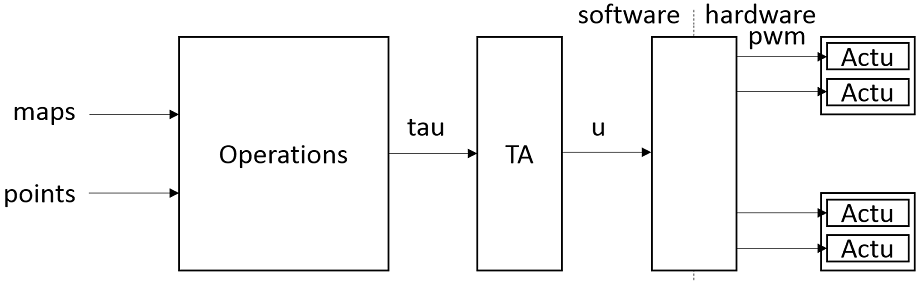
\includegraphics[scale=0.45]{fig/ctrl_operations} \caption{\label{fig: Marine Operations Control}Marine Operations Control}
\end{figure}

The more complex control modes, typically combined from several of
the different submodes, give automatic functions that are important
for different marine operations. Input varies depending on the operation.
It may be maps or waypoints, as in Figure \ref{fig: Marine Operations Control}.

Further details are discussed in Appendix \ref{subsec:Marine-Operations-Control}.


\part{Laboratory user guide}\label{part: Laboratory user guide}

\chapter{Safety and access}

\section{Hazards and measures}

\subsection{Personnel injury}

\paragraph{Drowning}
It is required to have two or more persons present when using the basin.

\paragraph{Electric shock}
The towing catenary should not be approached or touched.

\paragraph{Carriage collision}
It is forbidden to run the towing carriage when there are people alongside
the basin.

\paragraph{Thruster blade cuts}
Vessels must stay in the water as long as actuators are active. Before
removing the vessels from the water, the control system must be stopped
and disabled, for instance by undeploying in the VeriStand project.

\subsection{Material damage}

\paragraph{Cybership Enterprise 1}
\begin{description}
\item [{Water~damage:}] CSE1 is not waterproof and has excessive thrust capability which can inflict large roll angles. The risk of water on deck is reduced through thrust limitation and HIL testing before application of new control algorithms. 
\item [{Propeller~dry~running:}] BT must only be run in water. Before removing the vessel from the water, the control system must be stopped and the VeriStand project undeployed.
\item [{Loss~of~laptop~control:}] Wireless network instability may result in loss of connection between the laptop user interface and the cRIO. In this event, fall back to manual thruster control, by pushing 
\includegraphics[scale=0.4]{fig/sixaxis_triangle} on the Sixaxis.
\item [{Loss~of~position~measurement:}] -
\item [{Total~loss~of~control:}] Pull the vessel with a boat hook. Keep the CSE1 in water while disconnecting batteries.
\end{description}

\paragraph{Towing carriage}
Stop before automatic stop at high speeds.

\clearpage{}

\section{Access}
To access the laboratory, doors D-100, D-102 and D-316 are needed.
Door D-315 is also practical.

Get the necessary form from the NTNU reception. Deliver the form in
the Marintek reception.

\clearpage{}

\chapter{Qualisys motion capture system}\label{chap:Qualisys-motion-capture}
\section{Start Qualisys Track Manager}
\begin{enumerate}
\item Execute the program. The first displayed window is as in Figure \ref{fig: Qualisys Track Manager start window}.
\begin{figure}[!h]
\centering 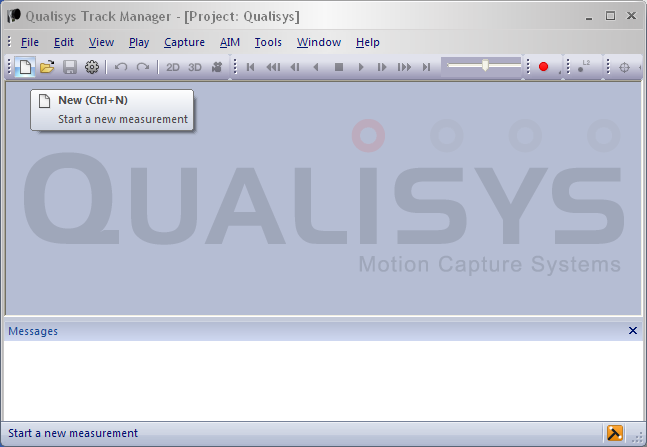
\includegraphics[width=1\textwidth]{fig/qualisys_new} \caption{\label{fig: Qualisys Track Manager start window}Qualisys Track Manager
start window}
\end{figure}
\item Push the white sheet icon to start a new measurement. The main window
should then display the 2D view, as in Figure \ref{fig: Qualisys Track Manager 2D view}.
\begin{figure}[!h]
\centering 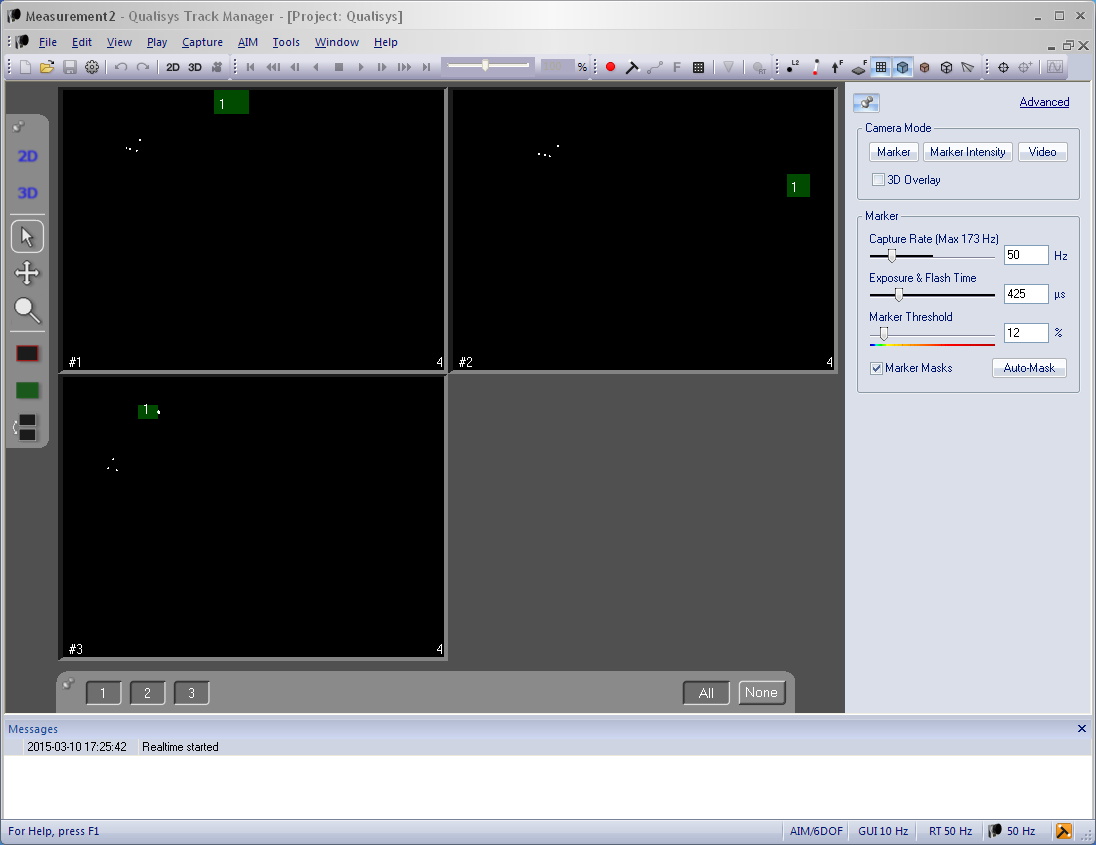
\includegraphics[width=1\textwidth]{fig/qualisys_3cams} \caption{\label{fig: Qualisys Track Manager 2D view}Qualisys Track Manager
2D view}
\end{figure}
 The squares numbered \#1, \#2 and \#3 show the basin as seen from
the respective cameras. The white dots are the vessel reflectors.
A minimum of three reflectors must be visible in each camera. 
\end{enumerate}

\section{Aquire body}
\begin{enumerate}
\item Push the gear icon to access Project Options. Navigate to 6DOF Tracking,
as in Figure \ref{fig:Qualisys-Track-Manager6DOF}.
\begin{figure}[!h]
\centering 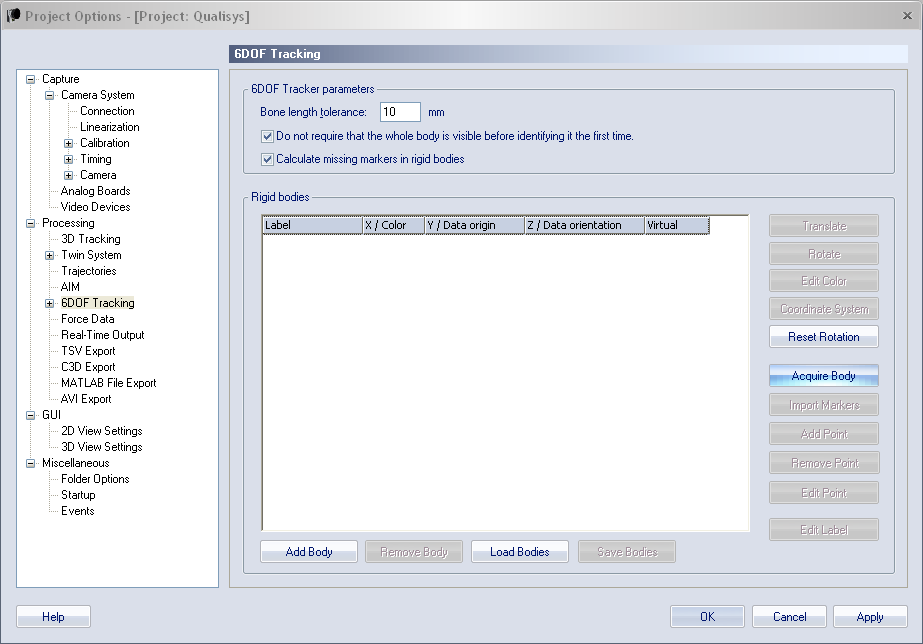
\includegraphics[width=1\textwidth]{fig/qualisys_6dof} \caption{\label{fig:Qualisys-Track-Manager6DOF}Qualisys Track Manager 6 DOF
Tracking}
\end{figure}
\item Remove previous bodies, if any.
\item Align the vessel with desired heading 0 and push ``Acquire Body''
to get the position of the reflectors. A list appears, as in Figure
\ref{fig:Qualisys-Track-ManagerAquiredBody}. 
\begin{figure}[!h]
\centering 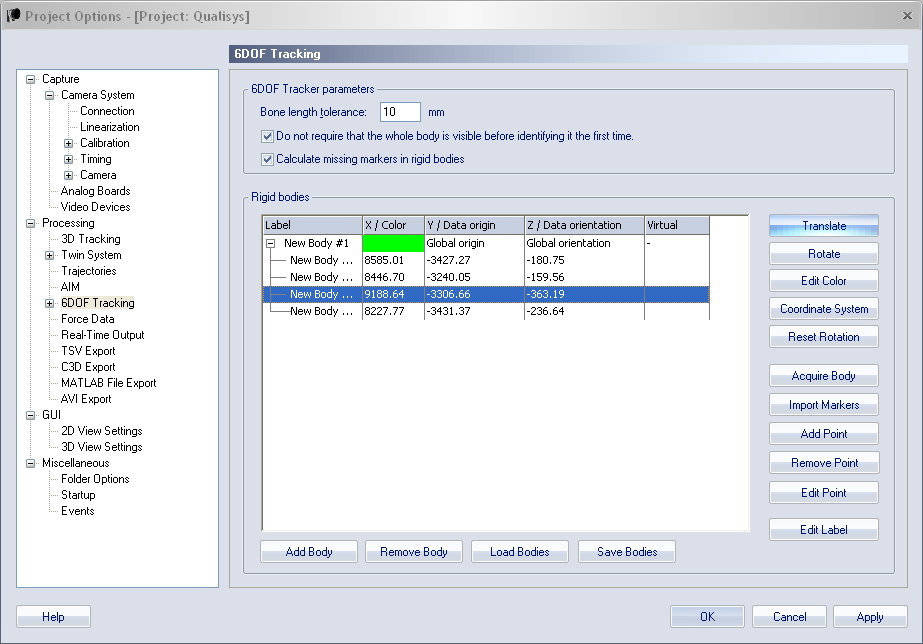
\includegraphics[width=1\textwidth]{fig/qualisys_orientating}
\caption{\label{fig:Qualisys-Track-ManagerAquiredBody}Qualisys Track Manager
aquired body}
\end{figure}
\item To redefine the body fixed coordinate frame 

\begin{enumerate}
\item Chose a reference reflector. As highlighted in Figure \ref{fig:Qualisys-Track-ManagerAquiredBody}, it may be practical to choose the highest-most, in this case reflector 3.
\item Push ``Translate'' and enter the coordinates of the chosen reflector in the desired frame. In Figure \ref{fig:Qualisys-Track-Managertranslate}, reflector 3 is set at $x,y,z=\left(0.550,0,-0.500\right)$. 
\begin{figure}[!h]
\centering 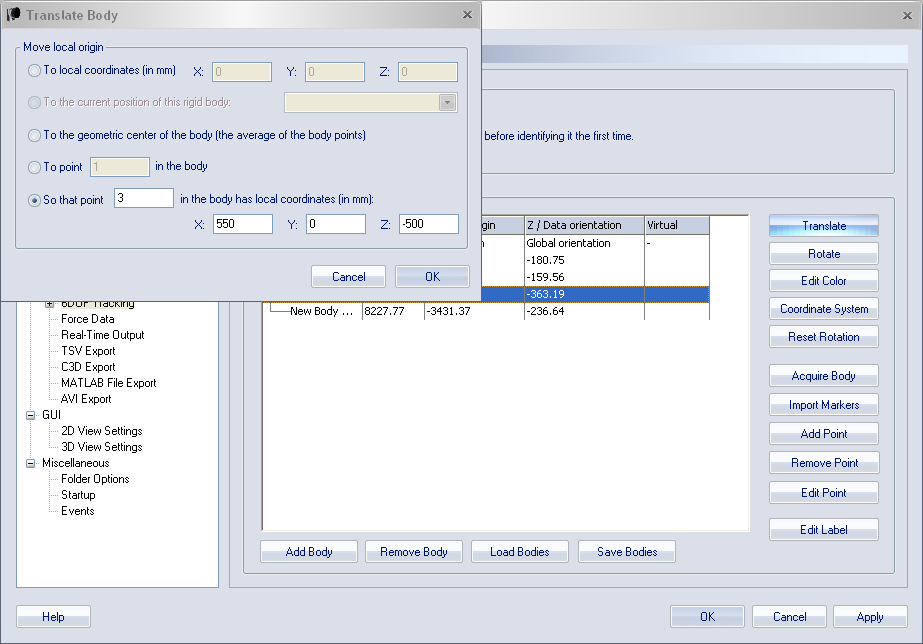
\includegraphics[width=1\textwidth]{fig/qualisys_orientating2}
\caption{\label{fig:Qualisys-Track-Managertranslate}Qualisys Track Manager
translate body}
\end{figure}
Figure \ref{fig:Qualisys-Track-Managertranslated} shows the resulting coordinates after translation.
\begin{figure}[!h]
\centering 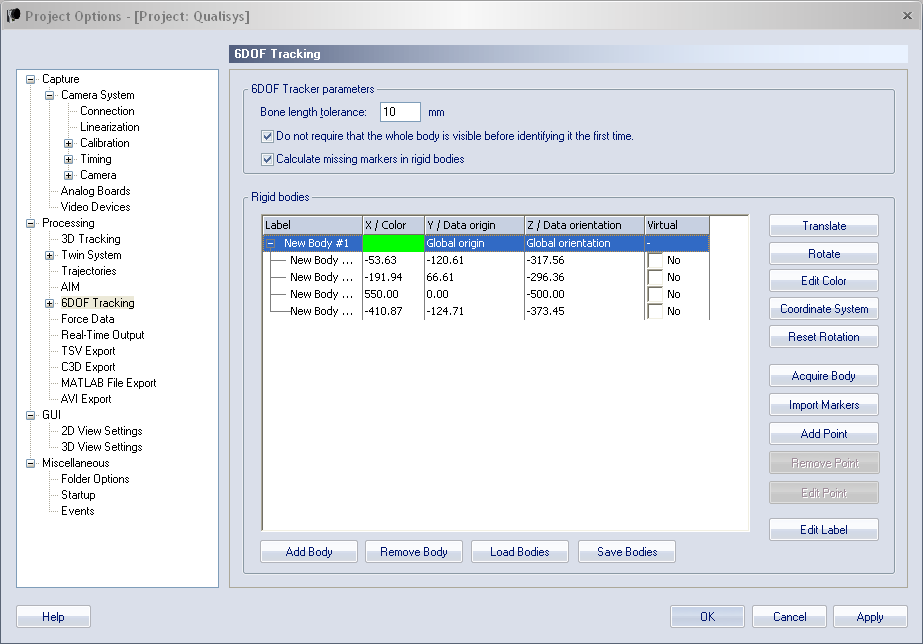
\includegraphics[width=1\textwidth]{fig/qualisys_orientating3}
\caption{\label{fig:Qualisys-Track-Managertranslated}Qualisys Track Manager translated body}
\end{figure}
\end{enumerate}
\item Finally, select 3D view to confirm that the body-fixed frame is indeed located as desired, as in Figure \ref{fig:Qualisys-Track-Managerr3D}.
\begin{figure}[!h]
\centering 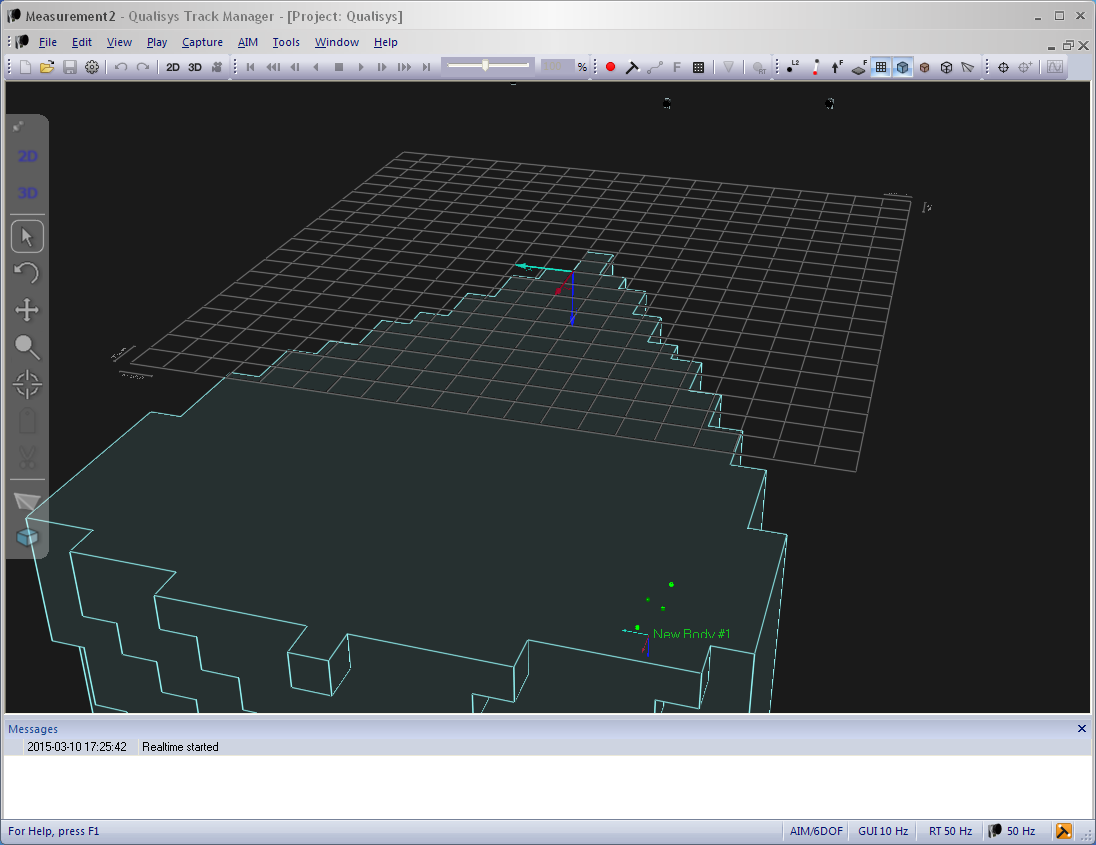
\includegraphics[width=1\textwidth]{fig/qualisys_3d} \caption{\label{fig:Qualisys-Track-Managerr3D}Qualisys Track Manager 3D view}
\end{figure}
\end{enumerate}

\section{Troubleshooting}
\subsection{Long waiting for camera}
\begin{figure}[!h]
\centering 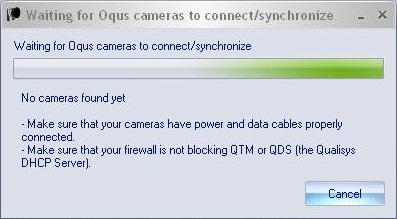
\includegraphics[scale=0.45]{fig/qualisys_waiting_to_connect}
\caption{\label{fig:Qualisys-Track-ManagerWaiting}Qualisys Track Manager waiting
for cameras}
\end{figure}
If the operation depicted in Figure \ref{fig:Qualisys-Track-ManagerWaiting}
is unsuccessful after a couple of minutes, reboot the cameras by unplugging
and reconnecting the power cord on the rack.

\clearpage{}

\section{Importing Data from the Qualisys System into ROS and MATLAB(Linux)}
The following approach may be used to read Qualisys data into ROS
and MATLAB. The method is convenient for Qualisys data into to MATLAB
independent on whether the rest of the system use ROS or not. The
method, as described is limited to Linux-operating systems.

The first part of the manual describe how import Qualisys data into
ROS, while the second part describe how to get the data from ROS into
MATLAB/Simulink.

Please note the following: 
\begin{itemize}
\item In the manual, the dollar sign \$ indicate a line of text that should
be written in the Linux- terminal window.
\item In the manual gedit is used as text editor. This can be replaced with
the readers favourite text editor.
\item The manual is written and tested for ROS-Indigo and MATLAB 2015b.
It is based on MATLAB's manual for importing custom messages \citep{MathWorks2016},
which is and adapted and expanded to fit that of the MC lab and the
Qualisys system.
\item You need MATLAB version 2015a or newer in order to proceed with the
MATLAB section of the manual.
\end{itemize}

\subsection{Manual}

If not already installed on the machine you should start by installing
ROS. Follow the instructions on the ROS download page: http://wiki.ros.org/indigo/Installation/Ubuntu

You should now make a ROS workspace in your home directory:

\begin{verbatim}$mkdir -p ~/catkin_ws/src 
$cd ~/catkin_ws/src
$catkin_init_workspace\end{verbatim}

You now need to make sure that one are sourcing the setup.bash file
in your ROS workspace each time you open your terminal window. This
can be done by changing the bash file with the following command:

\begin{verbatim}$ echo "source ~/catkin_ws/devel/setup.bash" >> ~/.bashrc\end{verbatim}

Now import the Qualisys driver from GitHub. (The driver \citep{KumarRobotics2016}
is avaiable through the Apache License )

\begin{verbatim}$ cd ~/catkin_ws/src
$ git clone https://github.com/KumarRobotics/qualisys
$ cd ~/catkin_ws
$ catkin_make\end{verbatim}

Open the qualisys.launch file in a text-editor

\begin{verbatim}$ sudo gedit ~/catkin_ws/src/qualisys/launch/qualisys.launch\end{verbatim}

Edit the ip address and port number for the Qualisys system. (As of
March 2016 the IP is: 192.168.0.10 and the port is 22222 )

The driver should now be set for interfacing with Qualisys in ROS.
To test it, first check that you are able to ping the Qualisys system
over the MC lab WiFi.

\begin{verbatim}$ ping 192.168.0.10\end{verbatim}

If you successfully pinged the qualisys system it should now be possible
to listen to the data from the Qualisys system.

(Note that the Qualisys system need to recognize the IR-markers in
the MC lab in order to transmit data. It may be smart to first to
check that the computer running Qualisys software in the MC-Lab sees
the marker)

\begin{verbatim}$ roslaunch qualisys qualisys.launch
$ rostopic list\end{verbatim}

The command ``rostopic list'' prints the ROS active ROS topics.
It should now be printed a qualisys topic in terminal. The name will
depend on the name set on the Qualisys computer. In this manual the
topic is named /qualisys/CSE1.

You can now listen to the data as it is published to ROS

\begin{verbatim}$ rostopic echo /qualisys/CSE1\end{verbatim}

\subsubsection{Getting Qualisys data to MATLAB}

The message sent from the Qualisys system is a custom message that
MATLAB does not recognize (most messages in ROS is not custom, and
will be recognized by MATLAB). In order to get the Qualisys data into
MATLAB you one to facilitate so that MATLAB recognize the custom message.

Start by creating a new folder \textasciitilde{}/qualisysDir. Now
copy the folder named qualisys, located in \textasciitilde{}/catkin\_ws/src
and paste it into the folder \textasciitilde{}/qualisysDir

Now one want to edit the package file so that MATLAB recognizes the
messages.

\begin{verbatim}Sudo gedit ~/qualisysDir/qualisys/package.xml\end{verbatim}

Add the following two lines somewhere in the main body of the package.xml
file.

\begin{verbatim}<build_depend>geometry_msgs</build_depend>
<build_depend>std_msgs</build_depend>\end{verbatim}

Now open MATLAB. The first step in MATLAB is to download the ROS custom
message package. Type the following lines into the MATLAB command
window, and follow instructions to download the ROS custom message
package.

\begin{verbatim}roboticsAddons (in MATLAB 2016)
roboticsSupportPackages  (in MATLAB 2015)\end{verbatim}

When the download is finished paste the following commands in the
MATLAB command window.

\begin{verbatim}folderpath= '~/qualisysDir'
rosgenmsg(folderpath)\end{verbatim}

Now follow the instructions generated by MATLAB in order generate
the needed message type. In this process you may need allow writing
permission to the file ``pathdef.m''

You are now ready to get the data into MATLAB.

Remember that the Qualisys node always need to be launched before
reading signals in MATLAB.

\begin{verbatim}roslaunch qualisys qualisys.launch\end{verbatim}

You can now get the data into Simulink by the Subscriber block, or
to MATLAB workspace by typing the following commands:

\begin{verbatim}Subb = rossubscriber('/qualisys/CSE1');
posedata = receive(Subb,10);\end{verbatim}

\clearpage{}

\chapter{Towing carriage}

\begin{figure}
\centering 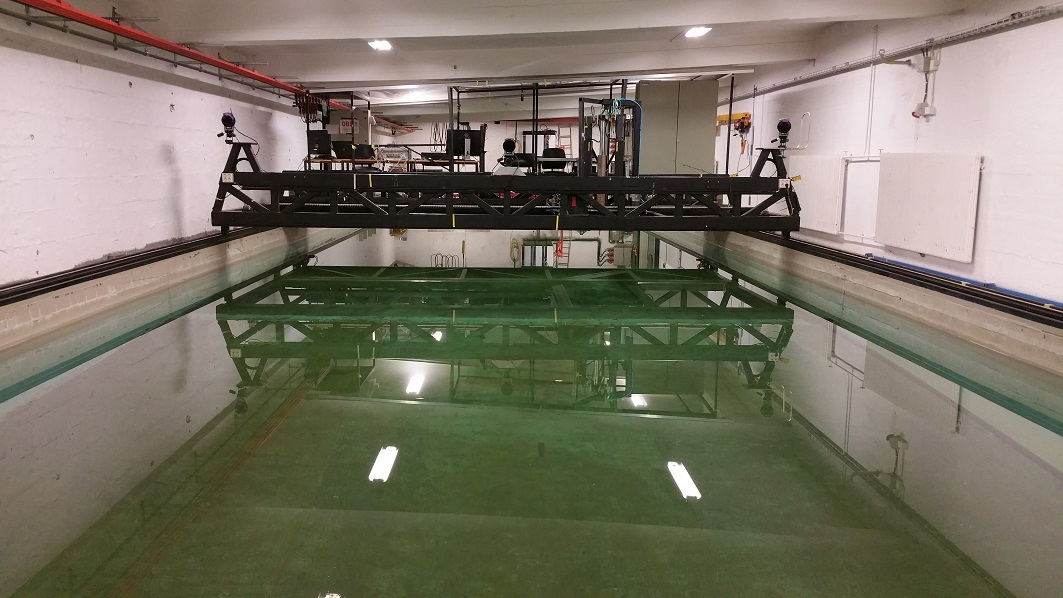
\includegraphics[width=1\textwidth]{fig/towing_carriage}
\caption{\label{fig: Towing carriage}Towing carriage}
\end{figure}

The scope of this section is to explain how to safely operate the
carriage without any damage towards humans or equipment. 

\section{Preparation before startup}

To start with, you must make sure that any items mounted or fixed
to the carriage are securely fitted, so they don't prevent the operation
of the carriage. All personnel must stay on the operation platform
during the travel of any axis.

Locate the Emergency Button and place it so that you can easily reach
it from where you are sited. DO NOT USE THE EMERGENCY BUTTOM AS A
BRAKE. YOU MUST ONLY OPERATE IT WHEN YOU ARE IN REAL EMERGENCY SITUATIONS.

\subsection{Operation console}

\begin{figure}
\centering 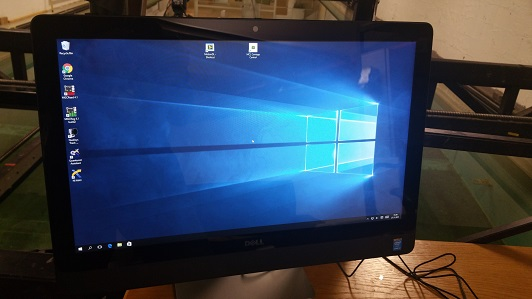
\includegraphics[width=0.8\textwidth]{fig/towing_console}
\caption{\label{fig: Towing console}Towing console}
\end{figure}

The operation console is an All-in-one PC. The Power button is on
the bottom right side of the screen. If the operation panel is not
on the desktop, you can start it by double clicking on desktop Icon,
shown in Figure \ref{fig: Towing console}.

\newpage{}

\section{Manual Operation of the Carriage}

\subsection{Setup}

\begin{figure}
\centering 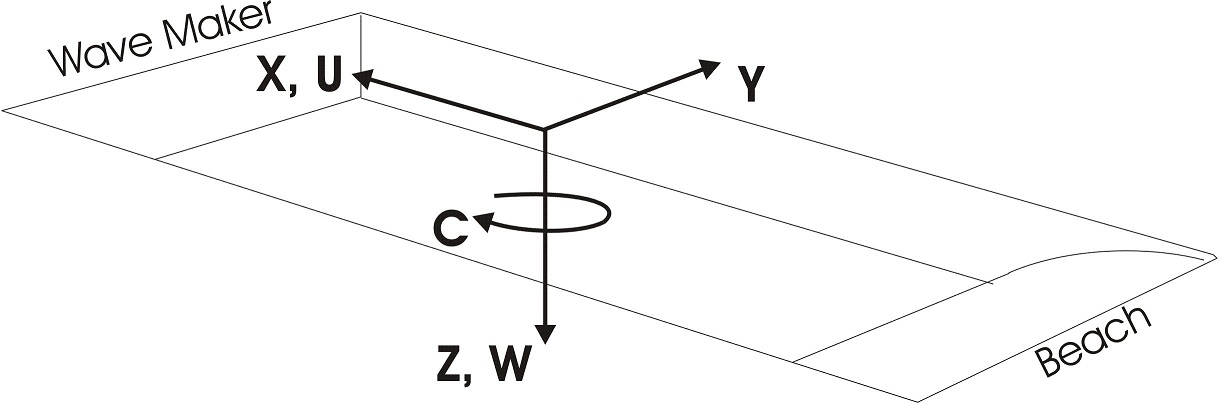
\includegraphics[width=0.8\textwidth]{fig/towing_coordinate_sketch}
\caption{\label{fig: Towing carriage-1}Coordinate system}
\end{figure}

\begin{figure}
\centering 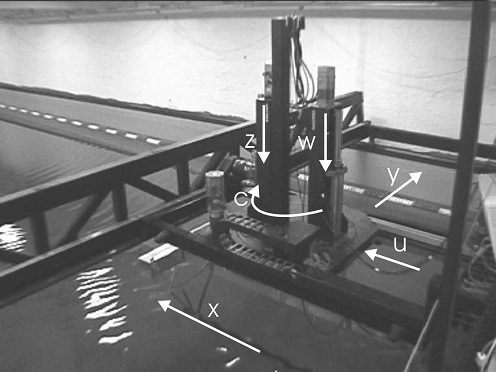
\includegraphics[width=0.8\textwidth]{fig/towing_coordinate_photo}
\caption{Coordinate system}
\end{figure}

\begin{table}
\centering{}%
\begin{tabular}{lllllll}
\hline 
 & \multicolumn{2}{l}{Forward/Backward} & \multicolumn{2}{l}{Acceleration} & \multicolumn{2}{l}{Position}\tabularnewline
Axis & \multicolumn{2}{l}{Speed} & \multicolumn{2}{l}{Deceleration} & \multicolumn{2}{l}{Pos./Neg. Limit}\tabularnewline
\hline 
X & 0 - 2.0 & {[}m/s{]}  & \% of 0 - 0.5 & $\text{m/\ensuremath{s^{2}}}$ & 0 - 22 & {[}m{]}\tabularnewline
Y & 0 - 1.0 & {[}m/s{]}  & \% of 0 - 1.0 & $\text{m/\ensuremath{s^{2}}}$ & 0 - 4.5 & {[}m{]}\tabularnewline
U & 0 - 1.0 & {[}m/s{]}  & \% of 0 - 1.0 & $\text{m/\ensuremath{s^{2}}}$ & 0 - 1 & {[}m{]}\tabularnewline
C & 0 - 10  & {[}deg/s{]} & \% of 0 - 20 & $\text{deg/\ensuremath{s^{2}}}$ & 0 - 255 & {[}deg{]}\tabularnewline
Z & 0 - 1.0 & {[}m/s{]}  & \% of 0 - 2.0 & $\text{m/\ensuremath{s^{2}}}$ & 0 - 0.5 & {[}m{]}\tabularnewline
W & 0 - 1.0 & {[}m/s{]}  & \% of 0 - 2.0 & $\text{m/\ensuremath{s^{2}}}$ & 0 - 0.5 & {[}m{]}\tabularnewline
\hline 
\end{tabular}\caption{\label{tab: Operation Limit}Operation Limit}
\end{table}

\begin{figure}
\centering 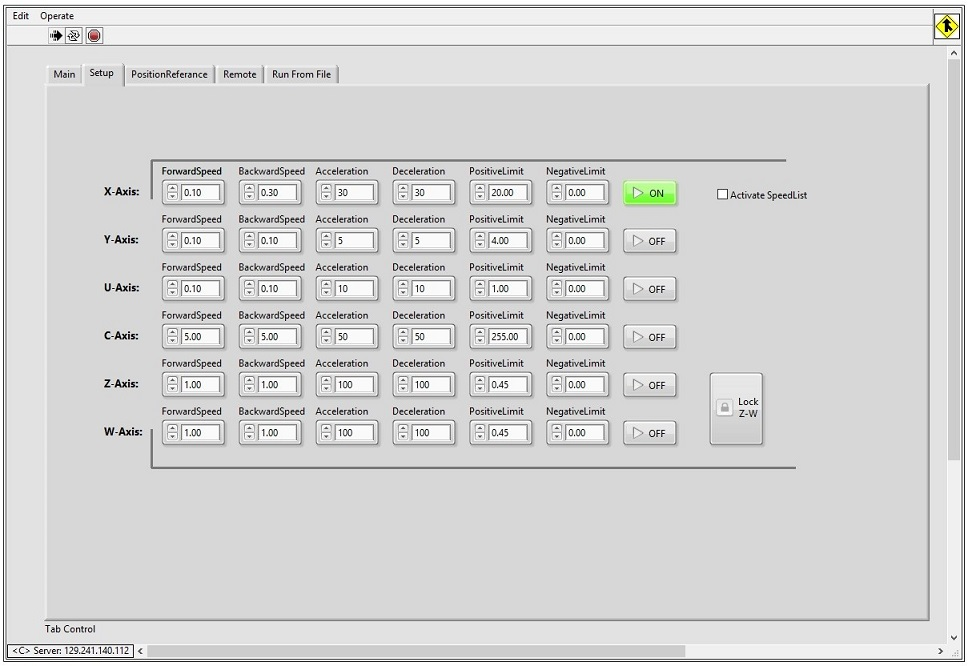
\includegraphics[width=0.8\textwidth]{fig/towing_parameteres}
\caption{\label{fig: Towing parameters}Setup}
\end{figure}

It is very important to select the Setup tab first before you start
any operation of the carriage. As you can see in Figure \ref{fig: Towing parameters},
it is possible to change the travel parameters for all available axes.
In principle, all axis parameters have different range limits. These
are listed in Table \ref{tab: Operation Limit}.

All axes can be activated or deactivate by using the ON button.

For the X axis it is possible to activate a list of predefined Forward
speeds. You will then have the ability to automatically change to
a different speed on the next run. The list can be edited in the Main
Tab Window.

By selecting the ``Lock Z-W'' button the Z-W axis will operate in
parallel. They will use the Z-axis parameter setup.

\subsection{Main/Standard Operation}

\begin{figure}
\centering 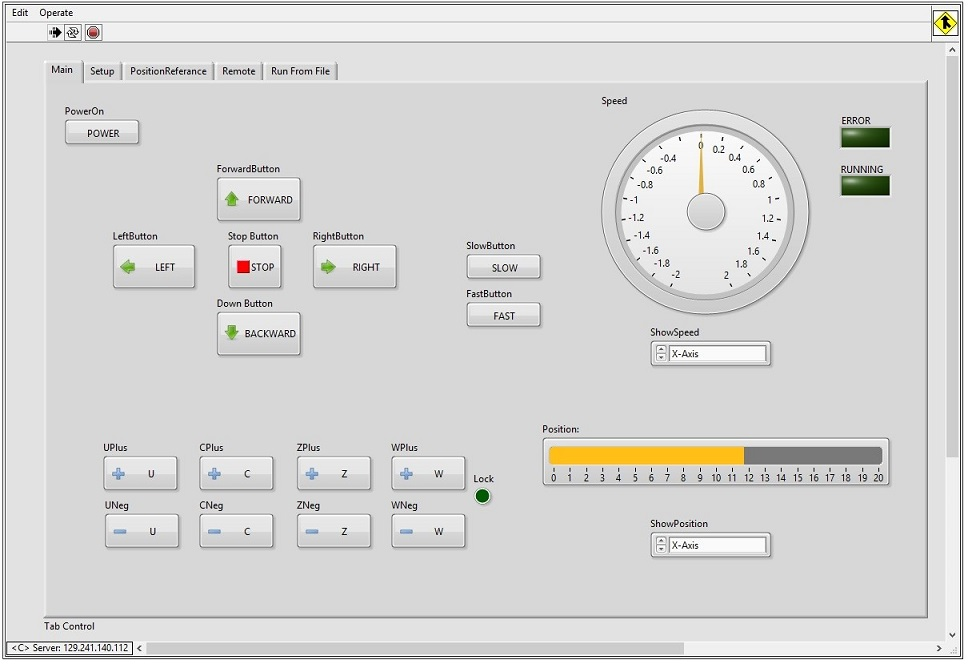
\includegraphics[width=0.8\textwidth]{fig/towing_main} \caption{\label{fig: Towing main}Main}
\end{figure}

All the activated axes will operate within the limits set in the Setup.
Only one axis can operate at a time. If you hit the button for another
axis than the running one, it will instantly stop and new one will
start running. To stop the running axis, simply hit the stop button.
If no buttons are operated carriage axis will run it hit limit position
of the current axis.

If an error occurs, for some reason, it can be cleared by hitting
the ``Power'' button. If the error keeps reoccurring, please look
at the Troubleshooting section of this document or contact responsible
MC Lab personnel.

The current speed and position of the active axis are displayed referred
to the selected limits.

\newpage{}

\section{Operation Controlled automatically from PC}

\begin{figure}
\centering 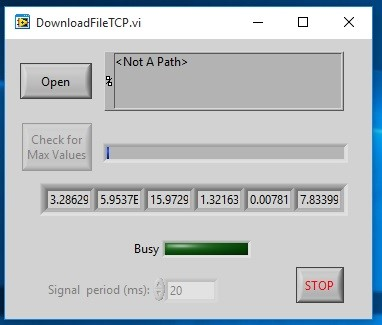
\includegraphics[width=0.8\textwidth]{fig/towing_runfromfile}
\caption{\label{fig: Towing main-1}Run From File}
\end{figure}


\subsection{The Trajectory Input File}

All trajectories must be defined in a .mcl input file. The format
of the file is slightly more general than allowed here and is the
same as for the sloshing rig input. The entries in the file are
\begin{enumerate}
\item Time Step in ms, double precision integer (int32). Must be set to
10.
\item Number of channels, double precision integer (int32). Must be 6.
\item Position references in sequence: X(1),Y(1),U(1),C(1),Z(1),W(1), X(2),Y(2),…
double precision real (float32).
\end{enumerate}
The following MTALAB lines write the matrix body (6xN) to file on
the correct format:

\begin{verbatim}
fid=fopen(filename,'wb');
head=[10;6];
count=fwrite(fid,head,'int32');
count=count+fwrite(fid,body,'float32');
fclose(fid); 
\end{verbatim}

The resulting input file must be transferred to the realtime computer
at /home/ntuser/inputpos.mcl. Normally this is done automatically
when the Load button on the LabVIEW GUI is pressed. 

\begin{figure}
\centering 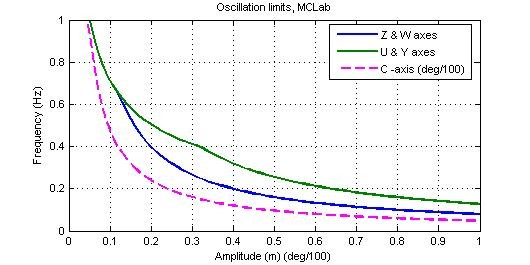
\includegraphics[width=0.8\textwidth]{fig/towing_ampvsfreq}
\caption{\label{fig: Towing main-1-1}Operation Limit Amplitude vs. Frequency}
\end{figure}

\newpage{}

\section{Troubleshooting}

-

\section{Note}

When the wagon is moving, no one is allowed to move on the sides of
the basin.

\clearpage{}

\section{Basic parameter identification}

\todo{Jon master}

\clearpage{}

\chapter{Wave generator}

\todo{Get basic information from Astrid, including hacking of wave
series}

\clearpage{}

\chapter{Current generator}

-

\clearpage{}

\chapter{CS Inocean Cat I Drillship}

\section{Mathematical model}

The proposed control design model is
\begin{eqnarray}
\dot{\eta} & = & R\left(\psi\right)\nu\label{eq: CSE1 kinematics-1}\\
M\dot{\nu} & = & -C\left(\nu\right)\nu-D\left(\nu\right)\nu+\tau\label{eq: CSE1 kinetics-1}
\end{eqnarray}
where
\begin{itemize}
\item the pose and velocity vectors are
\[
\eta=\left[\begin{array}{c}
x\\
y\\
\psi
\end{array}\right]\in\mathbb{R}^{3}\text{, and }\nu=\left[\begin{array}{c}
u\\
v\\
r
\end{array}\right]\in\mathbb{R}^{3},
\]
respectively. $\left(x,y\right)$ is the position and $\psi$ the
yaw angle or heading in the basin frame. $\left(u,v\right)$ are the
surge and sway velocities in the vessel frame, and $r$ is the yaw
rate.
\item the thrust force and moment vector is
\[
\tau=\left[\begin{array}{c}
X\\
Y\\
N
\end{array}\right]\in\mathbb{R}^{3},
\]
where $\left(X,Y\right)$ is the surge and sway force vector, and
$N$ is the yaw moment.
\item the three degrees of freedom (3 DOF) rotation matrix is
\[
R\left(\psi\right)=\left[\begin{array}{ccc}
\cos\psi & -\sin\psi & 0\\
\sin\psi & \cos\psi & 0\\
0 & 0 & 1
\end{array}\right].
\]
\item the vessel inertia matrix is
\[
M=\left[\begin{array}{ccc}
m-X_{\dot{u}} & 0 & 0\\
0 & m-Y_{\dot{v}} & mx_{g}-Y_{\dot{r}}\\
0 & mx_{g}-Y_{\dot{r}} & I_{z}-N_{\dot{r}}
\end{array}\right]=M^{\top}>0.
\]
 
\item the coriolis and centripetal matrix is
\begin{eqnarray*}
C\left(\nu\right) & = & \left[\begin{array}{ccc}
0 & 0 & -\left(m-Y_{\dot{v}}\right)v-\left(mx_{g}-Y_{\dot{r}}\right)r\\
mr & 0 & \left(m-X_{\dot{u}}\right)u\\
-\left(m-Y_{\dot{v}}\right)v-\left(mx_{g}-Y_{\dot{r}}\right)r & -\left(m-X_{\dot{u}}\right)u & 0
\end{array}\right]\\
 & = & -C^{\top}\left(\nu\right).
\end{eqnarray*}
\item the damping matrix is
\[
D\left(\nu\right)=-\left[\begin{array}{ccc}
d_{11}\left(u\right) & 0 & 0\\
0 & d_{22}\left(v,r\right) & d_{23}\left(v,r\right)\\
0 & d_{32}\left(v,r\right) & d_{33}\left(v,r\right)
\end{array}\right],
\]
where the damping components are 
\begin{eqnarray}
d_{11}\left(u\right) & = & X_{u}+X_{\left\vert u\right\vert u}\left\vert u\right\vert +X_{uuu}u^{2}<0\label{Eq:d11-1}\\
d_{22}\left(v,r\right) & = & Y_{v}+Y_{\left\vert v\right\vert v}\left\vert v\right\vert +Y_{vvv}v^{2}<0\label{Eq:d22-1}\\
d_{23}\left(v,r\right) & =\label{Eq:d23-1}\\
d_{32}\left(v,r\right) & =\label{Eq:d32-1}\\
d_{33}\left(v,r\right) & = & N_{r}+N_{\left\vert r\right\vert r}\left\vert r\right\vert +N_{rrr}r^{2}<0\label{Eq:d33-1}
\end{eqnarray}
\end{itemize}
\begin{table}
\begin{centering}
\begin{tabular}{crcr}
\multicolumn{2}{c}{Rigid body} & \multicolumn{2}{c}{Added mass}\tabularnewline
\midrule 
Parameter & Value & Parameter & Value\tabularnewline
\midrule 
$m$  &  & $X_{\dot{u}}$  & \tabularnewline
$I_{z}$  &  & $Y_{\dot{v}}$  & \tabularnewline
$x_{g}$  &  & $Y_{\dot{r}}$  & \tabularnewline
$y_{g}$  &  & $N_{\dot{r}}$  & \tabularnewline
\bottomrule
\end{tabular}
\par\end{centering}
\caption{\label{tab: CSE1-rigid-body-1}Rigid body and added mass parameters}
\end{table}

The rigid body inertia and hydrodynamic added mass parameters are
given in Table \ref{tab: CSE1-rigid-body-1}.

\begin{table}
\begin{centering}
\begin{tabular}{lrrlrrlr}
\multicolumn{2}{c}{Surge} &  & \multicolumn{2}{c}{Sway} &  & \multicolumn{2}{c}{Yaw}\tabularnewline
\midrule 
$X_{u}$  & $-2.332$  &  & $Y_{v}$  & $-4.673$  &  & $N_{v}$  & JON\tabularnewline
$X_{\left|u\right|u}$  & $0.000$  &  & $Y_{\left|v\right|v}$  & $0.3976$  &  & $N_{\left|v\right|v}$  & JON\tabularnewline
$X_{uuu}$  & $-8.557$  &  & $Y_{vvv}$  & $-313.3$  &  & $N_{vvv}$  & JON\tabularnewline
\bottomrule
\end{tabular}
\par\end{centering}
\caption{\label{tab: CSE1 damping parameters 2-1}CSE1 damping parameters}
\end{table}

The hydrodynamic damping parameters are given in Tables \ref{tab: CSE1 damping parameters 1-1}
and \ref{tab: CSE1 damping parameters 2-1}.

The model is valid for low-speed.

The thrust forces and moments ranges are listed in Table \ref{tab: CSEI Thust Moment-1}.
\begin{table}
\begin{centering}
\begin{tabular}{lrllrl}
 & \multicolumn{2}{c}{Thrust} &  & \multicolumn{2}{c}{Velocity}\tabularnewline
\midrule 
Surge & $X$ & JON {[}N{]} &  & $u$ & JON {[}m/s{]}\tabularnewline
Sway & $Y$ & JON {[}N{]} &  & $v$ & JON {[}m/s{]}\tabularnewline
Yaw & $N$ & JON {[}N$\cdot$m{]} &  & $r$ & JON {[}rad/s{]}\tabularnewline
\bottomrule
\end{tabular}
\par\end{centering}
\caption{\label{tab: CSEI Thust Moment-1}Model validity range}
\end{table}

\todo{Add material from Jon}

\clearpage{}

\chapter{CS Enterprise I}

\section{Mathematical model}

The proposed control design model is
\begin{eqnarray}
\dot{\eta} & = & R\left(\psi\right)\nu\label{eq: CSE1 kinematics}\\
M\dot{\nu} & = & -C\left(\nu\right)\nu-D\left(\nu\right)\nu+\tau\label{eq: CSE1 kinetics}
\end{eqnarray}
where
\begin{itemize}
\item the pose and velocity vectors are
\[
\eta=\left[\begin{array}{c}
x\\
y\\
\psi
\end{array}\right]\in\mathbb{R}^{3}\text{, and }\nu=\left[\begin{array}{c}
u\\
v\\
r
\end{array}\right]\in\mathbb{R}^{3},
\]
respectively. $\left(x,y\right)$ is the position and $\psi$ the
yaw angle or heading in the basin frame. $\left(u,v\right)$ are the
surge and sway velocities in the CSE1 vessel frame, and $r$ is the
yaw rate.
\item the thrust force and moment vector is
\[
\tau=\left[\begin{array}{c}
X\\
Y\\
N
\end{array}\right]\in\mathbb{R}^{3},
\]
where $\left(X,Y\right)$ is the surge and sway force vector, and
$N$ is the yaw moment. The thrust forces and moments ranges are listed
in Table \ref{tab: CSEI Thust Moment}.
\begin{table}
\begin{centering}
\begin{tabular}{cc}
 & Max\tabularnewline
\midrule 
Surge $X$  & $1.03$ N\tabularnewline
Sway $Y$  & $2.50$ N\tabularnewline
Yaw $N$  & $0.98$ N\tabularnewline
\bottomrule
\end{tabular}
\par\end{centering}
\caption{\label{tab: CSEI Thust Moment}CSEI forces and moments given $\omega_{\text{VSP}}=0.3$}
\end{table}
\item the three degrees of freedom (3 DOF) rotation matrix is
\[
R\left(\psi\right)=\left[\begin{array}{ccc}
\cos\psi & -\sin\psi & 0\\
\sin\psi & \cos\psi & 0\\
0 & 0 & 1
\end{array}\right].
\]
\item the vessel inertia matrix is
\[
M=\left[\begin{array}{ccc}
m-X_{\dot{u}} & 0 & 0\\
0 & m-Y_{\dot{v}} & mx_{g}-Y_{\dot{r}}\\
0 & mx_{g}-Y_{\dot{r}} & I_{z}-N_{\dot{r}}
\end{array}\right]=M^{\top}>0.
\]
 
\item the coriolis and centripetal matrix is
\[
C\left(\nu\right)=\left[\begin{array}{ccc}
0 & -mr & Y_{\dot{v}}v+\left(Y_{\dot{r}}-mx_{g}\right)r\\
mr & 0 & -X_{\dot{u}}u\\
-Y_{\dot{v}}v-\left(Y_{\dot{r}}-mx_{g}\right)r & X_{\dot{u}}u & 0
\end{array}\right]=-C^{\top}\left(\nu\right).
\]
\item the damping matrix is
\[
D\left(\nu\right)=\left[\begin{array}{ccc}
d_{11}\left(u\right) & 0 & 0\\
0 & d_{22}\left(v,r\right) & d_{23}\left(v,r\right)\\
0 & d_{32}\left(v,r\right) & d_{33}\left(v,r\right)
\end{array}\right],
\]
where the damping components are 
\begin{eqnarray}
d_{11}\left(u\right) & = & -X_{u}-X_{\left\vert u\right\vert u}\left\vert u\right\vert -X_{uuu}u^{2}\label{Eq:d11}\\
d_{22}\left(v,r\right) & = & -Y_{v}-Y_{\left\vert v\right\vert v}\left\vert v\right\vert -Y_{vvv}v^{2}-Y_{\left\vert r\right\vert v}\left\vert r\right\vert \label{Eq:d22}\\
d_{23}\left(v,r\right) & = & -Y_{r}-Y_{\left\vert v\right\vert r}\left\vert v\right\vert -Y_{\left\vert r\right\vert r}\left\vert r\right\vert -Y_{rrr}r^{2}\label{Eq:d23}\\
d_{32}\left(v,r\right) & = & -N_{v}-N_{\left\vert v\right\vert v}\left\vert v\right\vert -N_{vvv}v^{2}-N_{\left\vert r\right\vert v}\left\vert r\right\vert \label{Eq:d32}\\
d_{33}\left(v,r\right) & = & -N_{r}-N_{\left\vert v\right\vert r}\left\vert v\right\vert -N_{\left\vert r\right\vert r}\left\vert r\right\vert -N_{rrr}r^{2}\label{Eq:d33}
\end{eqnarray}
\end{itemize}

\begin{table}
\begin{centering}
\begin{tabular}{crcr}
\multicolumn{2}{c}{Rigid body} & \multicolumn{2}{c}{Added mass}\tabularnewline
\midrule 
Parameter & Value & Parameter & Value\tabularnewline
\midrule 
$m$  & $14.79$  & $X_{\dot{u}}$  & $-2$ \tabularnewline
$I_{z}$  & $1.76$  & $Y_{\dot{v}}$  & $-10$ \tabularnewline
$x_{g}$  & $0.0375$  & $Y_{\dot{r}}$  & $-0$ \tabularnewline
$y_{g}$  & $0.0$  & $N_{\dot{r}}$  & $-1$ \tabularnewline
\bottomrule
\end{tabular}
\par\end{centering}
\caption{\label{tab: CSE1-rigid-body}CSE1 rigid body and added mass parameters}
\end{table}

The rigid body inertia and hydrodynamic added mass parameters are
given in Table \ref{tab: CSE1-rigid-body}.

\begin{table}
\begin{centering}
\begin{tabular}{crcrcr}
\multicolumn{2}{c}{Hydro surge} & \multicolumn{2}{c}{Hydro sway} & \multicolumn{2}{c}{Hydro yaw}\tabularnewline
\midrule 
{Parameter}  & {Value}  & {Parameter}  & {Value}  & {Parameter}  & {Value} \tabularnewline
\midrule 
$X_{u}$  & $-0.6555$  & $Y_{v}$  & $-1.33$  & $N_{v}$  & $0.0$ \tabularnewline
$X_{uu}$  & $0.3545$  & $Y_{vv}$  & $-2.776$  & $N_{vv}$  & $-0.2088$ \tabularnewline
$X_{uuu}$  & $-3.787$  & $Y_{vvv}$  & $-64.91$  & $N_{vvv}$  & $0.0$ \tabularnewline
$X_{v}$  & $0.0$  & $Y_{r}$  & $-7.25$  & $N_{r}$  & $-1.9$ \tabularnewline
$X_{vv}$  & $-2.443$  & $Y_{rr}$  & $-3.45$  & $N_{rr}$  & $-0.75$ \tabularnewline
$X_{vvv}$  & $0.0$  & $Y_{rrr}$  & $0.0$  & $N_{rrr}$  & $0.0$ \tabularnewline
$.$  & $.$  & $Y_{rv}$  & $-0.805$  & $N_{rv}$  & $0.130$ \tabularnewline
$.$  & $.$  & $Y_{vr}$  & $-0.845$  & $N_{vr}$  & $0.080$ \tabularnewline
\bottomrule
\end{tabular}
\par\end{centering}
\caption{\label{tab: CSE1 damping parameters 2}CSE1 damping parameters}
\end{table}

The hydrodynamic damping parameters are given in Tables \ref{tab: CSE1 damping parameters 1}
and \ref{tab: CSE1 damping parameters 2}.

The model is valid for low-speed.

\clearpage{}

\section{Model-in-the-loop simulation}

\clearpage{}

\section{Processor-in-the-Loop simulation}

\begin{figure}
\centering 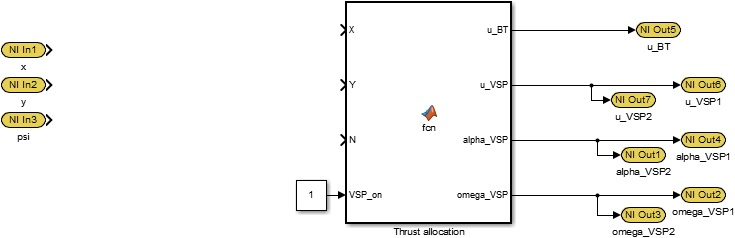
\includegraphics[scale=0.45]{fig/CSE1_ctrl_student} \caption{\label{fig: CSE1 ctrl_student.slx}CSE1 \texttt{ctrl\_student.slx}
including thrust allocation}
\end{figure}

Implementation of the student controller is done in the \texttt{ctrl\_student.slx}
Simulink template, depicted in Figure \ref{fig: CSE1 ctrl_student.slx}.
Detailed implementation steps are given in Section \ref{sec: CSE1 Student controller implementation}.

The generic control system consists of several Simulink modules, the
details of which are given in Appendix \ref{subsec: CSE1 Control software},
a FPGA driver, described in Appendix \ref{subsec:Create-FPGA-target},
and two custom device drivers.

\clearpage{}

\section{Basin testing}

\subsection{\label{sec: CSE1 Student controller implementation}Student controller
implementation}
\begin{enumerate}
\item Download the control system from GitHub\\
{\texttt{github.com/NTNU-MCS/CS\_EnterpriseI\_cRIO}} 
\item Unzip the control system. The prefered path is \texttt{C:\textbackslash{}CS\_EnterpriseI\_cRIO\textbackslash{}}.
Other paths require updating paths in the project definition.
\item Simulink implementation and compilation

\begin{enumerate}
\item Update {\texttt{ctrl\_student.slx}} according to your controller
design. Additional input and output, resets and data logging may be
added, as described in Section \ref{subsec: Simulink modeling}.\\
Do not alter the predefined input and output: x\_m, y\_m, psi\_m,
u\_BT, u\_VSP1, u\_VSP2, alpha\_VSP1, alpha\_VSP2, omega\_VSP1 and
omega\_VSP2.
\item Select a suitable solver, as described in Section \ref{subsec: Simulink model configuration}.\\
The remaining configuration, such as target selection is preselected
in the file.
\item Compile the model as described in Section \ref{subsec: Simulink model build}.
If using the prefered path, the MATLAB current folder should be \texttt{C:\textbackslash{}CS\_EnterpriseI\_cRIO\textbackslash{}simulink
source\textbackslash{}}, in order to ensure that the resulting \texttt{.out}
file is created in \texttt{C:\textbackslash{}CS\_EnterpriseI\_cRIO\textbackslash{}simulink
source\textbackslash{}ctrl\_student\_niVeriStand\_VxWorks\_rtw}.
\end{enumerate}
\item CSE1 VeriStand Project configuration

\begin{enumerate}
\item Open {\texttt{CSE1.nivsproj}}\footnote{Not \texttt{CSE1.nivssdf}, since not only the system definition should
be altered.} to access the project.
\item Update {\texttt{ctrl\_student.out}}:

\begin{enumerate}
\item Open the System Explorer by double-clicking the system definition
file \texttt{CSE1.nivssdf}.
\item 
\begin{figure}
\centering 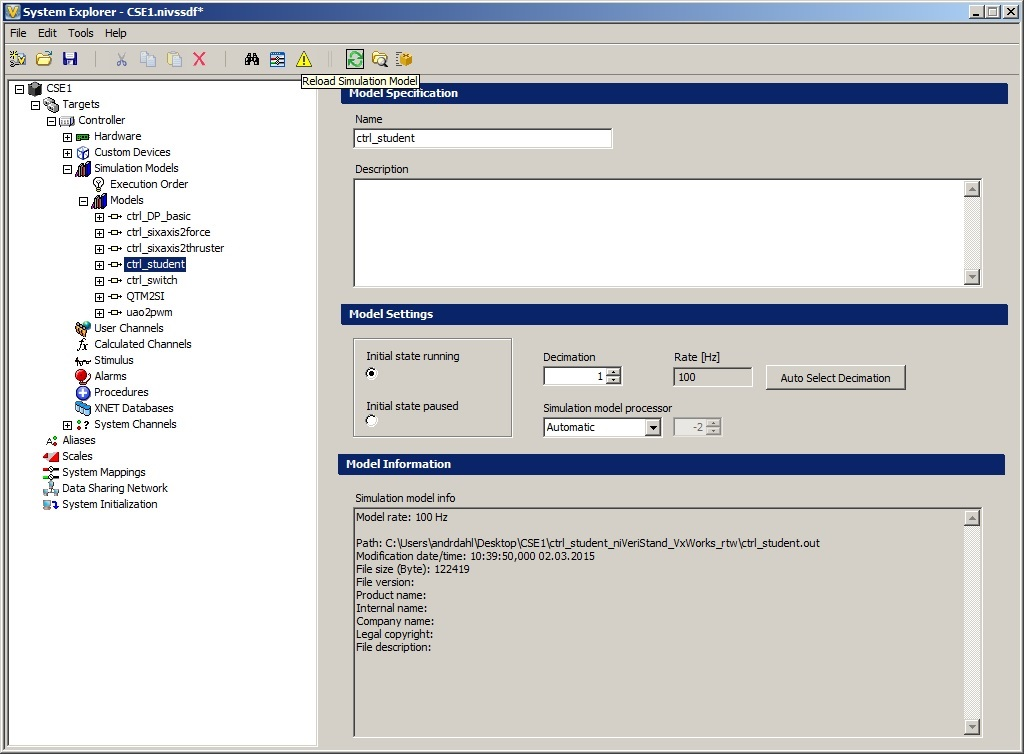
\includegraphics[scale=0.45]{fig/CSE1_update_ctrl_studtent}
\caption{\label{fig: CSE1 simulation models}CSE1 Veristand Project simulation
models}
\end{figure}
Browse the left pane tree, as seen in Figure \ref{fig: CSE1 simulation models},
and select ctrl\_student. Refresh by pushing the 
\includegraphics[scale=0.8]{fig/veristand_refresh}
icon.
\item If necessary, add mappings.\\
Do not change the existing mappings. Position input (x, y, psi) and
controller output (u\_BT, u\_VSP1, u\_VSP2, alpha\_VSP1, alpha\_VSP2,
omega\_VSP1, omega\_VSP2) are already mapped as necessary.
\item Save and close to return to the Project Explorer.
\end{enumerate}
\item 
\begin{figure}
\centering 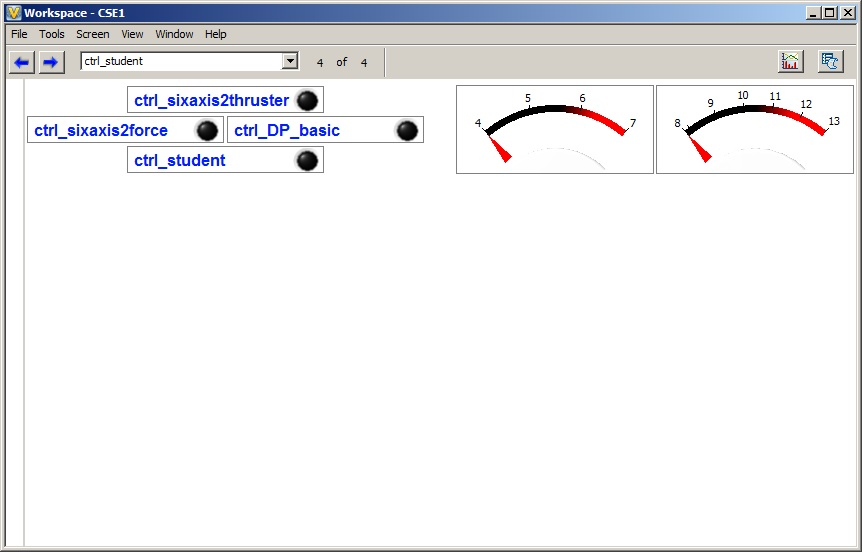
\includegraphics[scale=0.45]{fig/CSE1_student_workspace}
\caption{\label{fig: CSE1 student_ctrl workspace}CSE1 Veristand Project ctrl\_student
workspace}
\end{figure}
Implement a suitable workspace, as described in Section \ref{subsec: Create computer interface},
for your controller in control screen 4: ctrl\_student. Figure \ref{fig: CSE1 student_ctrl workspace}
shows control screen 4 before customization.
\end{enumerate}
\end{enumerate}
\clearpage{}

\subsection{Ship launching procedure - before sailing}

\subsubsection{Power up and connection}
\begin{enumerate}
\item Place the batteries adjacent to the watertight box: main battery (12
V) astern, a secondary battery (6 V) in the bow and a third battery
(6V) just behind the main battery, see Figure \ref{fig:CSE1-Second6V}.
\item Connect main battery: first the red wire to the red/positive pole,
then the black wire to the black/negative pole\footnote{The connection order of the wires should not matter. However, experiences
favor the this order of connection.}.\\
cRIO LED nr.1 (power) will light up green.
\item Wait for cRIO and RPi start up.\\
When complete, the Bluetooth dongle blue LED blinks evenly at approximately
1 Hz.
\item Turn on Sixaxis by pushing the PS3 button.\\
When succesfully connected, the Bluetooth dongle blue LED is almost
constantly lit and the Sixaxis' red LEDs 1, 2, 3, and 4 blink at approximately
2 Hz.
\item Connect the seconday and the third battery: red wire to the red/positive
pole, then the black wire to the black/negative pole.\\
The Wifi bridge Power LED will light up green.
\item Wait for WiFi connection to HILlab network.\\
When connected, the Wifi bridge WLAN green LED turns on.
\item 
\begin{figure}[h]
\centering 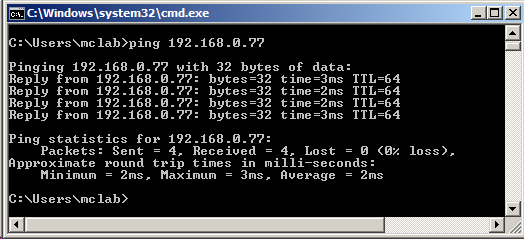
\includegraphics[scale=0.45]{fig/cRIO_ping} \caption{\label{fig: ping}Ping, successful access to CSE1}
\end{figure}
Verify laptop access: ping the CSE1 IP in the command promt, as in
Figure \ref{fig: ping}. While the round trip times may vary, it is
essential to have 0\% loss.
\item Gently place the vessel in the basin, avoiding any water splashes.
\end{enumerate}


\subsubsection{Positioning system}

If the positioning system is not initialized for CSE1, follow the
procedures in Chapter \ref{chap:Qualisys-motion-capture}.

\clearpage{}

\subsection{Deploy control system}

\todo{Veristand osv}

A diagram representation of CSE1's control system is given in Figure
\ref{fig: CSE1 generic control system}. The first three controllers
are predefined, while users may implement their own controller in
the fourth.

\begin{table}
\centering{}%
\begin{tabular}{c>{\raggedright}p{6.5cm}}
\hline 
Sixaxis & Control mode\tabularnewline
\hline 

\includegraphics[scale=0.4]{fig/sixaxis_triangle} & \textbf{Manual thruster control}

VSP speed: directional pad up/down $\pm0.1$

Left joystick: VSP1 thrust

Right joystick: VSP2 thrust

L2/R2: BT thrust\tabularnewline
\hline 

\includegraphics[scale=0.4]{fig/sixaxis_square} & \textbf{Manual forces and moment control}

VSP speed: user interface button on/off

Left joystick: surge and sway forces

L2/R2: yaw moment\tabularnewline
\hline 

\includegraphics[scale=0.4]{fig/sixaxis_circle} & \textbf{Basic dynamic positioning (DP)}

VSP speed: user interface button on/off

Setpoint: user interface

Gains: user interface\tabularnewline
\hline 

\includegraphics[scale=0.4]{fig/sixaxis_cross} & \textbf{Student controller}

User implemented controller\tabularnewline
\hline 
\end{tabular}\caption{\label{tab: CSE1 control system modes}Generic control modes}
\end{table}

The vessel can switch among four control modes, summarized in Table
\ref{tab: CSE1 control system modes}. 

\clearpage{}

\subsection{Ship docking procedure - after sailing}

Undeploy the running project to disable all actuators.

Lift out of water avoiding water on rail.

Put CSE1 in its stand. The vessel should not be left on the water
for extensive periods, i.e. overnight.

Remove and put used batteries to charge. Load fresh batteries in vessel.

Connect the Sixaxis gamepad to the laptop for charging.

\clearpage{}

\subsection{Troubleshooting}

-

\FloatBarrier

\clearpage{}

\chapter{CS Saucer}

\section{Required Software}

NI LabVIEW software required to run the project ``CyberShip Saucer'':
\begin{enumerate}
\item LabVIEW 2014
\item LabVIEW 2014 myRIO Toolkit
\item LabVIEW 2014 Real-Time Module
\item LabVIEW Control Design and Simulation Module
\end{enumerate}

\section{Deployment}

When the power source is connected and the Wi indicator lights up,
the vessel is ready to deploy.
\begin{itemize}
\item Run the host application ``mainHost.vi''.
\item Deploy the target application ``main.vi''.
\end{itemize}
The vessel is now operational.

\section{NI Dashboard Manual Control}

The CS Saucer can be controlled directly from an Android or a iOS
device with the NI Dashboard app.

\section{Manual Thruster Control}
\begin{itemize}
\item Make sure that your device is connected to the local are network with
a static ip adress.
\item Create a new Dashboard with six slide controls, these will be the
six control inputs $u_{0}$, $u_{1}$, $u_{2}$, $\alpha_{0}$, $\alpha_{1}$
and $\alpha_{2}$.
\item Congure the scale of the slide controls so that $u\in\left[-1,1\right]$
and $\alpha\in\left[-114,114\right]$
\item Tap a control to connect it to its corresponding shared variable node
on the myRIO. The ip adress for the myRIO-Saucer is: 192:168:0:99.
\item The shared variable nodes for the manual thruster control are located
in the library ``libctrlMaualThruster''. Be careful to only use
the variables with the label ``DSH''.
\item Start the dashboard.
\end{itemize}

\section{Manual Force Control}
\begin{itemize}
\item Make sure that your device is connected to the local are network with
a static ip adress.
\item Create a new Dashboard with three slide controls, this will be the
commanded force vector $\tau=\left[X,Y,N\right]^{\top}$.
\item Congure the scale of the slide controls so that $X=\left[-9;9\right]$,
$Y=\left[-9;9\right]$ and $N=\left[-4;4\right]$
\item Tap a control to connect it to its corresponding shared variable node
on the myRIO. The ip adress for the myRIO-Saucer is: 192:168:0:99.
\item The shared variable nodes for the manual force control are located
in the library ``libctrlMaualForce''. Be careful to only use the
variables with the label ``DSH''.
\item Start the dashboard.
\end{itemize}

\section{Data logging}

\begin{figure}[h]
\centering 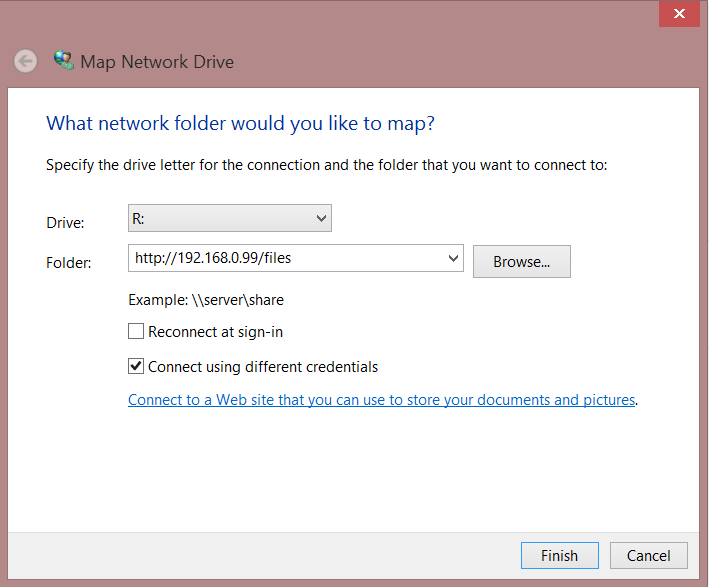
\includegraphics[scale=0.45]{fig/Saucer_mapnetworkdrive}
\caption{\label{fig: Saucer map network}Map network drive to the NI myRIO.}
\end{figure}
\begin{figure}[h]
\centering 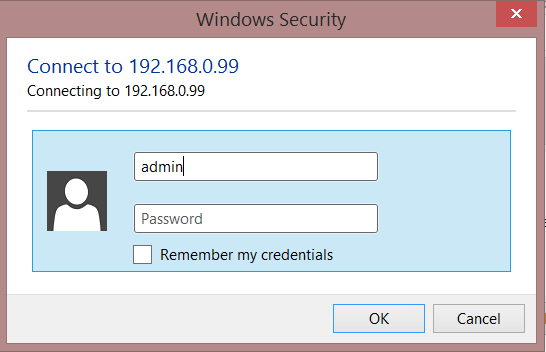
\includegraphics[scale=0.45]{fig/Saucer_credentials} \caption{\label{fig: Saucer credentials}Login credentials on the myRIO-Saucer.
The password is blank.}
\end{figure}
\begin{figure}[h]
\centering 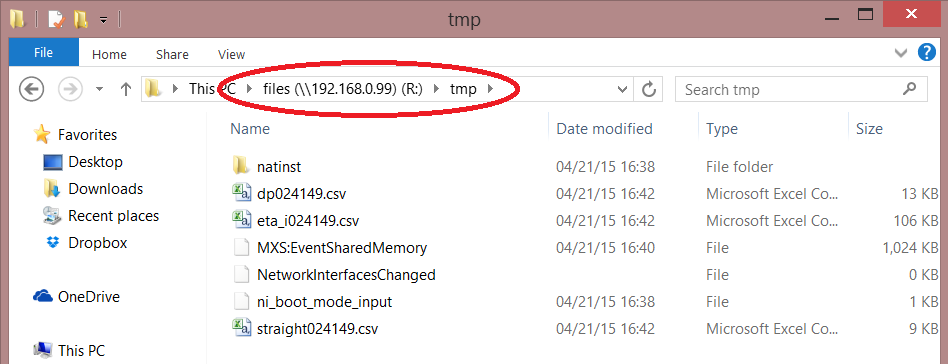
\includegraphics[scale=0.45]{fig/saucer_logfiles} \caption{\label{fig: Saucer log files}The log les are saved in the tmp folder
on the myRIO}
\end{figure}

Continuous data logging has been implemented in the main target application.
On initialization, a ``.csv'' le is created for each of the control
modes. The log le for a control mode will only be populated when that
particular control mode is active. Each log le is created with a control
mode identier and a time stamp, e.g. ``dp114700''. The log le format
``.csv'' (comma separated values) is highly compatible with MATLAB
and enables easy import and post processing of the data in MATLAB.
The import code in the script is easily created using MATLAB's import
le wizard which generates code for le import for a specic le.

The log les on the myRIO are stored in the ``les/tmp'' folder which
is a temporary folder that is cleared on reboot. Saving the log les
in this directory ensures that the target does not use all of its
storage memory to store old log les. A log le can be easily exported
from the target by using the ``Map network drive'' feature in Windows.
Simply map to the static ip of the target as shown in Figure \ref{fig: Saucer map network}.
Remember to check the ``Connect using dierent credentials'' box.
When prompted for a password, type in ``admin'' as the user and
leave the password blank as shown in Figure \ref{fig: Saucer credentials}.
The ``les/tmp'' directory of the target is now available in the
windows le explorer as seen in Figure \ref{fig: Saucer log files}.

\section{Charging the Traxxas LiPo Battery}

Connect both the balancing plug and the main power plug to the charger
before starting a charge. Then place the battery in the ame resistant
bag. Ensure that the charger is set to LiPo mode before pressing start.
The charging indicator will turn green when the battery is fully charged.

Discharging the battery lower than 9V can destroy it or lead to reduced
capacity and performance. It is therefore recommended that the battery
should be charged when reaching a voltage of 11.1. The voltage of
the battery can be measured with a voltmeter on the balancing plug.
Using the ground wire in the balancing plug, the voltage of each of
the cells can be measured from three remaining wires in the plug.
If the LiPo battery is discharged below 9V it will not charge in LiPo
mode. It is therefor wise to stay well above this limit. Should this
happen, the battery can be charged in ``NIMh'' mode for maximum
10 seconds. This has proved to be eective for getting the voltage
above 9V and able to charge in LiPo mode again. However it should
be stressed that this measure be used with extremea caution and only
as a last resort.

\clearpage{}

\chapter{ROV Neptunus}

k

\clearpage{}

\newpage{}

\part{Laboratory Staff Guide}\label{part: Equipment setup and configuration}

\chapter{cRIO-based control system setup}

\section{\label{subsec: cRIO setup}cRIO}

The cRIO runs Wind River VxWorks real-time operating system.

\subsection{Ethernet ports}

The cRIO has two Ethernet ports the primary communicates with the
PC and the secondary with the Raspberry PI.

\subsubsection{Primary}

Set fixed IP, set fixed IP on HIL-computers

\subsubsection{Enabling the secondary ethernet port}

\begin{enumerate}
\item Start \emph{NI MAX}
\item In the left pane tree, select the cRIO under \emph{Remote Systems}
\item Open the \emph{Network Settings} tab (located at the bottom of the
window)
\item Set \emph{Adapter Mode} to \emph{TCP/IP Network}
\item Set \emph{Configure IPv4 Address} to \emph{Static}
\end{enumerate}
\begin{figure}[!h]
\centering 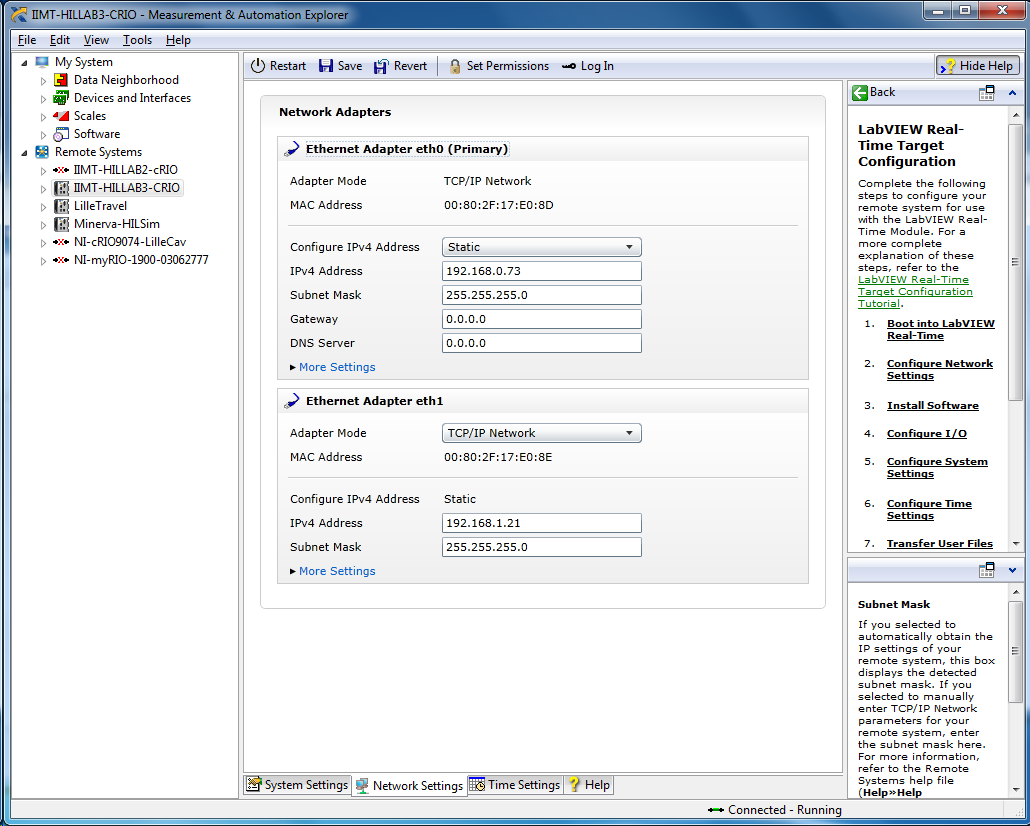
\includegraphics[scale=0.45]{Screenshots/Screenshot_2015-01-16_14-10-14.png}
\caption{NI MAX - Network Settings}

\label{fig: network settings} 
\end{figure}

\FloatBarrier

\newpage{}

\subsection{Update cRIO software}

To be able to run the models on the cRIO, the software version on
the cRIO and PC must match. In addition you must install the NI Veristand
Engine. Software changes on the cRIO is handled in NI Max.

\subsubsection{Update}
\begin{enumerate}
\item Open NI Max
\item Find your cRIO on the left hand side and click it
\item Click Software, and then Add/Rem ove Software located on the top pane,
see Figure \ref{fig: Software update 1}
\item A new window will now open. Choose the option that matches your LabVIEW/Veristand
edition (in our case 14.0 or 14.0.1) under LabVIEW Real-Time 14.0.0
and click next. See Figure \ref{fig: NI MAX - Software Update 2}
\item Click next without making any changes\ref{fig: NI MAX - Software Update 1-3}
\item Click next without making any changes\ref{fig: NI MAX - Software Update 4}
\item Wait for the installtion to finish and the cRIO to reboot
\end{enumerate}
\begin{figure}[!h]
\centering 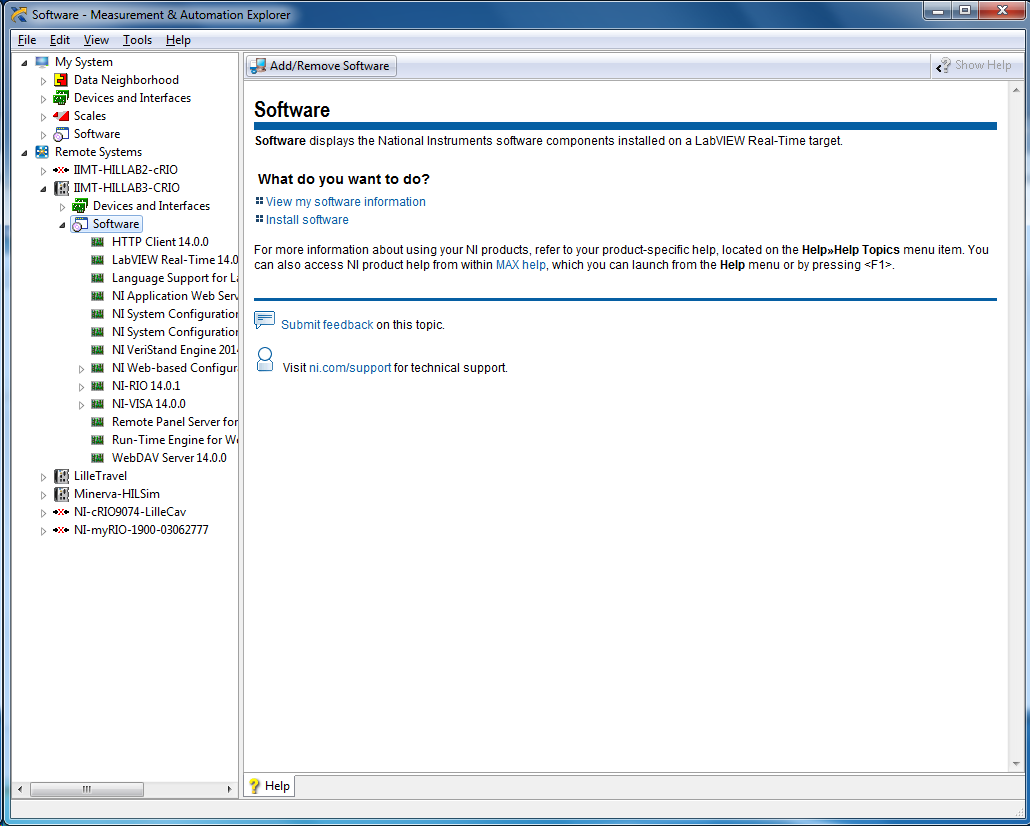
\includegraphics[scale=0.45]{Screenshots/Screenshot_2015-01-16_14-12-35.png}
\caption{NI MAX - Software Update 1}

\label{fig: Software update 1} 
\end{figure}

\begin{figure}[!h]
\centering 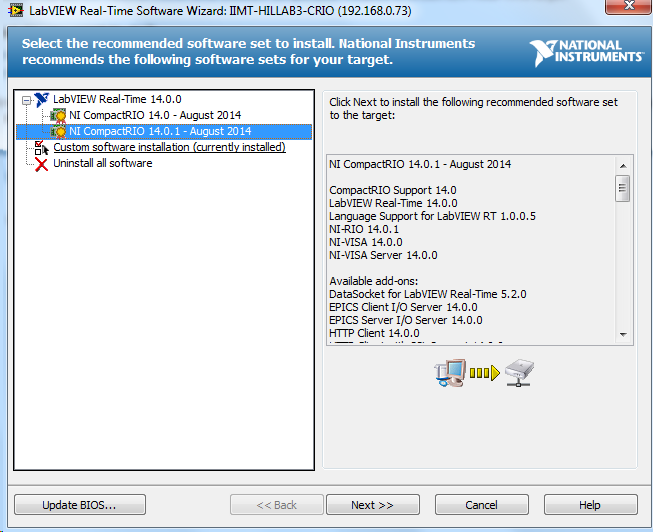
\includegraphics[scale=0.45]{Screenshots/Screenshot_2015-01-16_14-12-51.png}
\caption{NI MAX - Software Update 1}

\label{fig: NI MAX - Software Update 2} 
\end{figure}

\begin{figure}[!h]
\centering 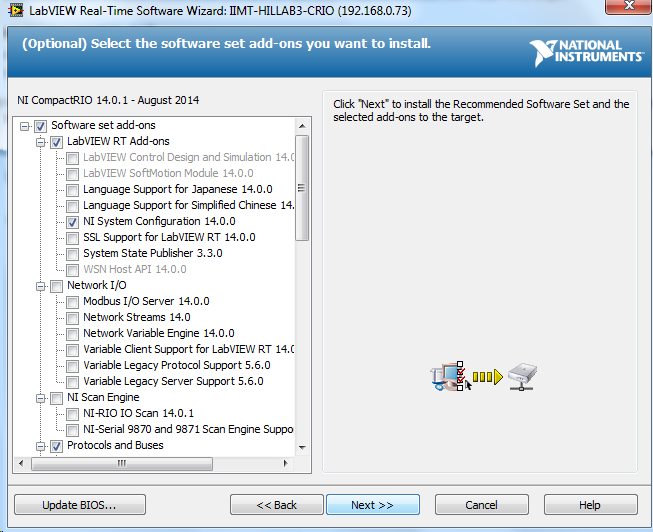
\includegraphics[scale=0.45]{Screenshots/Screenshot_2015-01-16_14-13-03.png}
\caption{NI MAX - Software Update 3}

\label{fig: NI MAX - Software Update 1-3} 
\end{figure}

\begin{figure}[!h]
\centering 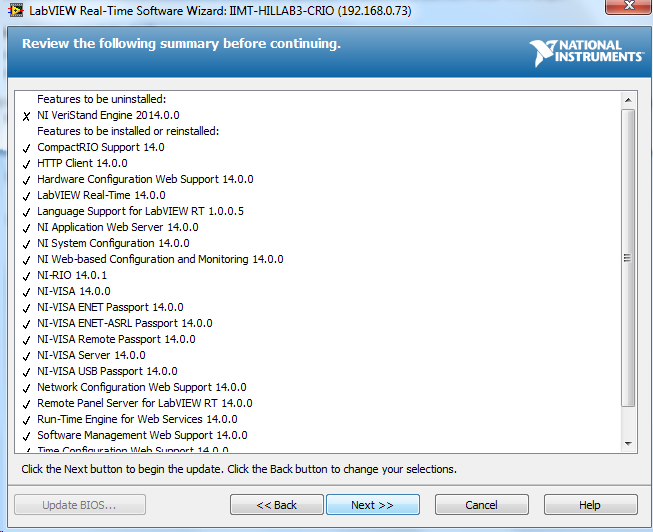
\includegraphics[scale=0.45]{Screenshots/Screenshot_2015-01-16_14-15-22.png}
\caption{NI MAX - Software Update 4}

\label{fig: NI MAX - Software Update 4} 
\end{figure}

\FloatBarrier

\subsubsection{NI Veristand Engine}
\begin{enumerate}
\item Repeat step 1-3 from the previous guide
\item Now you choose Custom Software installation in the menu, see Figure
\ref{fig: NI Veristand Engine installation 1}
\item Ignore the warning, See Figure \ref{fig: NI Veristand Engine installation 1-1}
\item Locate NI Veristand Engine 2014 0.0 and click install feature. See
Figure \ref{fig: NI Veristand Engine installation 1-2}
\item Click your way through the rest of the installation and let the cRIO
reboot.
\end{enumerate}
\begin{figure}[!h]
\centering 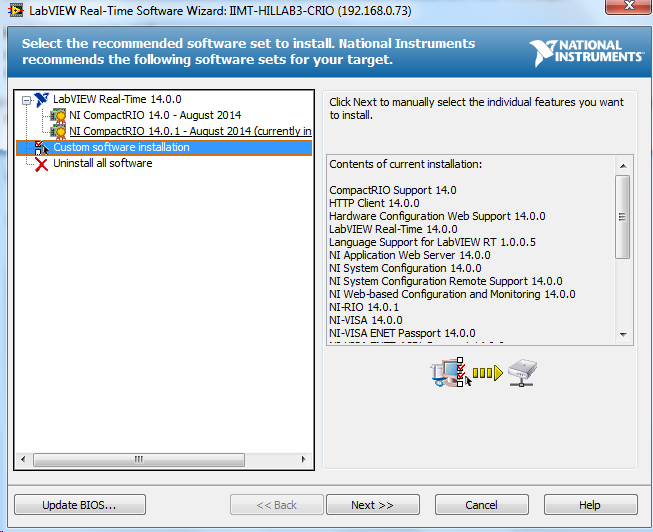
\includegraphics[scale=0.45]{Screenshots/Screenshot_2015-01-16_14-20-27.png}
\caption{NI MAX - NI Veristand Engine installation 1}

\label{fig: NI Veristand Engine installation 1} 
\end{figure}

\begin{figure}[!h]
\centering \includegraphics[scale=0.45]{Screenshots/Screenshot_2015-01-16_14-20-39.png}
\caption{NI MAX - NI Veristand Engine installation 1}

\label{fig: NI Veristand Engine installation 1-1} 
\end{figure}
\begin{figure}[!h]
\centering \includegraphics[scale=0.45]{Screenshots/Screenshot_2015-01-16_14-21-07.png}
\caption{NI MAX - NI Veristand Engine installation 1}

\label{fig: NI Veristand Engine installation 1-2} 
\end{figure}

\clearpage{}

\subsection{\label{subsec:Create-FPGA-target}Create FPGA target and XML}

If you do not haav a Veristand FPGA target at your disposal, follow
the steps below. If you have a target available and just need to install
it in NI Veristand, please jump to the next subsection
\begin{enumerate}
\item Open LabVIEW and create new project. We have done this in LabVIEW
2013 because of some instalation issues with LabVIEW 2014, but the
procedure should be the same for both editions.
\item Choose NI Veristand FPGA Project in project templates and proceed.
\item Choose CompactRIO Reconfiguarble Embedded System and click next.
\item You will now get the choice between letting LabVIEW detect your cRIO
system or configure it yourself. If you are connected to the cRIO
and it has all of the I/O ports connected, the option ``Discover
existing system'' is simpler and therefore recommneded. If you do
not have your cRIO connected choose ``Create new system'', this
is the version that will be worked through here.
\item Select your controller, in our case cRIO-9024.
\item Select your FPGA target, in our case cRIO-9113.
\item Then you select your I/O modules to the correct slots. In our case
NI 9215 in slot 1 and NI 9474 in slot 4.
\item You are now finished with configuring your project. Press next.
\item The project menu will now appear and should look something like Figure
\ref{fig: Create Labview FPGA target and XML-10}. Select the LabVIEW
VI as demonstrated our is called Custom Personality FPGA.vi
\item The UI window will now present itself, select window and show block
diagram.
\item You should now see a block diagram similar to Figure \ref{fig: Create Labview FPGA target and XML-11}.
You will now have to redesign this to look like Figure \ref{fig: Create Labview FPGA target and XML-12}.
This will be valid for our system, if you have different I/O modules
the block diagram need to reflect this.
\item Now, return to the Project explorer and select Build Specifications
and Custom Personality FPGA
\item A new window will open. Check that the name and project path is correct
and press build.
\item Select your preferred compile server. The compilation process will
take quite some time (approx 15-30 min).
\item When the compilation process is finished, the last step is to edit
the automatically generated XML file. You will now have to find you
project directory in Windows. Here there will be a folder called bitfiles
which contains the files you compiled in the last step, there will
also be a .XML file. The point of editing this file is to match the
actually compiled VI, meaning the packets must match the connected
I/O. The recommended way to edit the file is to copy our XML file
from: Dropbox\textbackslash{}TMR4243 - LAB\textbackslash{}04 cRIO
software\textbackslash{}FPGA IO. You will have to make sure that the
name of your bitfile matches the name in the XML file as seen in Figure
\ref{fig: Create Labview FPGA target and XML-17}, also make sure
the I/O modules matches your setup.
\item Copy the bitfiles from the bitfile folder to the level above so that
the bitfile aand the XML file is in the same folder.
\end{enumerate}
Documentation: \url{https://decibel.ni.com/content/docs/DOC-13815}

\begin{figure}[!h]
\centering \includegraphics[scale=0.45]{Screenshots/Screenshot_2015-01-16_19-21-16.png}
\caption{Create Labview FPGA target and XML - 1}

\label{fig: Create Labview FPGA target and XML-1} 
\end{figure}

\begin{figure}[!h]
\centering \includegraphics[scale=0.45]{Screenshots/Screenshot_2015-01-16_19-23-23.png}
\caption{Create Labview FPGA target and XML - 2}

\label{fig: Create Labview FPGA target and XML-2} 
\end{figure}

\begin{figure}[!h]
\centering \includegraphics[scale=0.45]{Screenshots/Screenshot_2015-01-16_19-23-41.png}
\caption{Create Labview FPGA target and XML - 3}

\label{fig: Create Labview FPGA target and XML-3} 
\end{figure}

\begin{figure}[!h]
\centering \includegraphics[scale=0.45]{Screenshots/Screenshot_2015-01-16_19-23-58.png}
\caption{Create Labview FPGA target and XML -4}

\label{fig: Create Labview FPGA target and XML-4} 
\end{figure}

\begin{figure}[!h]
\centering \includegraphics[scale=0.45]{Screenshots/Screenshot_2015-01-16_19-24-31.png}
\caption{Create Labview FPGA target and XML - 5}

\label{fig: Create Labview FPGA target and XML-5} 
\end{figure}

\begin{figure}[!h]
\centering \includegraphics[scale=0.45]{Screenshots/Screenshot_2015-01-16_19-24-43.png}
\caption{Create Labview FPGA target and XML - 6}

\label{fig: Create Labview FPGA target and XML-6} 
\end{figure}

\begin{figure}[!h]
\centering \includegraphics[scale=0.45]{Screenshots/Screenshot_2015-01-16_19-25-37.png}
\caption{Create Labview FPGA target and XML - 7}

\label{fig: Create Labview FPGA target and XML-7} 
\end{figure}

\begin{figure}[!h]
\centering \includegraphics[scale=0.45]{Screenshots/Screenshot_2015-01-16_19-25-54.png}
\caption{Create Labview FPGA target and XML - 8}

\label{fig: Create Labview FPGA target and XML-8} 
\end{figure}

\begin{figure}[!h]
\centering \includegraphics[scale=0.45]{Screenshots/Screenshot_2015-01-16_19-28-17.png}
\caption{Create Labview FPGA target and XML -9}

\label{fig: Create Labview FPGA target and XML-9} 
\end{figure}

\begin{figure}[!h]
\centering \includegraphics[scale=0.45]{Screenshots/Screenshot_2015-01-16_19-28-41.png}
\caption{Create Labview FPGA target and XML - 10}

\label{fig: Create Labview FPGA target and XML-10} 
\end{figure}

\begin{figure}[!h]
\centering \includegraphics[angle=-90,scale=0.45]{Screenshots/Screenshot_2015-01-16_19-29-04.png}
\caption{Create Labview FPGA target and XML - 11}

\label{fig: Create Labview FPGA target and XML-11} 
\end{figure}

\begin{figure}[!h]
\centering \includegraphics[angle=-90,scale=0.45]{Screenshots/Screenshot_2015-01-16_20-07-43.png}
\caption{Create Labview FPGA target and XML - 12}

\label{fig: Create Labview FPGA target and XML-12} 
\end{figure}

\begin{figure}[!h]
\centering \includegraphics[scale=0.45]{Screenshots/Screenshot_2015-01-16_19-52-25.png}
\caption{Create Labview FPGA target and XML - 13}

\label{fig: Create Labview FPGA target and XML-13} 
\end{figure}

\begin{figure}[!h]
\centering \includegraphics[scale=0.45]{Screenshots/Screenshot_2015-01-16_19-53-01.png}
\caption{Create Labview FPGA target and XML - 14}

\label{fig: Create Labview FPGA target and XML-14} 
\end{figure}

\begin{figure}[!h]
\centering \includegraphics[scale=0.45]{Screenshots/Screenshot_2015-01-16_19-53-25.png}
\caption{Create Labview FPGA target and XML - 15}

\label{fig: Create Labview FPGA target and XML-15} 
\end{figure}

\begin{figure}[!h]
\centering \includegraphics[scale=0.45]{Screenshots/Screenshot_2015-01-16_20-01-32.png}
\caption{Create Labview FPGA target and XML - 16}

\label{fig: Create Labview FPGA target and XML-16} 
\end{figure}

\begin{figure}[!h]
\centering \includegraphics[scale=0.45]{Screenshots/Screenshot_2015-01-17_13-59-31.png}
\caption{Create Labview FPGA target and XML - 17}

\label{fig: Create Labview FPGA target and XML-17} 
\end{figure}

Veristand FPGA programmering

In order to access the analogue and digital I/O modules on our cRIO
from Veristand, it is necessary to create a FPGA target in Labview
with Labview and you will have to write a custom XML file.

\subsubsection{Install in veristand}

The Veristand software does not recognize the physical I/O components
of the cRIO. It is necessarry to write a specific FPGA mapping for
the specific setup. This results in a XML file that maps the ports. 

To add this file to your Veristand project, enter the system explorer
and find the FPGA pane under \textit{targets\textbackslash{}controller\textbackslash{}hardware\textbackslash{}chassis},
as seen in figure \ref{fig: fpga1}. 

\begin{figure}[!h]
\centering \includegraphics[scale=0.45]{fig/fpga1}

\caption{FPGA1}

\label{fig: fpga1}
\end{figure}

The next step is to find your XML file. In this case called cRIO-9113
Ex, it is very important that the XML file is placed on level above
the FPGA bitfile folder in the directory system, as the files are
really being used are the FPGA bitfiles.

\begin{figure}[!h]
\centering \includegraphics[scale=0.45]{fig/fpga2}

\caption{FPGA2}

\label{fig: fpga2}
\end{figure}

The menu in should now look something like Figure \ref{fig: fpga2},
here you can see the analogue input signals and the digital output
PWM signals. These can again be linked to other signals as seen in
Figure\ref{fig: veristand mappings}.

\begin{figure}
\includegraphics[scale=0.45]{fig/fpga3}

\caption{FPGA3}

\label{fig: fpga3}
\end{figure}

PWM

\paragraph{Ticks og sånt}

tick = FPGA clock pulse

\[
\text{tick in seconds}=\frac{1}{\text{frequency}}=\frac{1}{40MHz}=\frac{1}{40*10^{6}}=25*10^{-}9=25ns
\]

output at 50 Hz demands output every 
\[
\frac{40MHz}{50Hz}=\frac{40*10^{6}}{50}=800000tick
\]


\paragraph{VeriStand FPGA programming}

LabView -\textgreater{} Create project -\textgreater{} All -\textgreater{}
NI VeriStand FPGA project -\textgreater{} Compact RIO -\textgreater{}
Discover existing system -\textgreater{} Velge eget utstyr -\textgreater{}
Vente på discovering -\textgreater{} I Project explorer {*}.vi (er
bitfilen) {*}.fpgaconfig (egentlig XML) Endre på {*}.vi Fjerne overføldige
pakker Oppdatere antall pakker i XML-filen og fjerne pakker som ikke
er aktuelle, oppdatere tall på beholdte pakker. Kompiler

Kopier bit-file ut i samme mappe som {*}.fpgaconfig I System exlporer,
FPGA -\textgreater{} Add FPGA target -\textgreater{} Finne {*}.fpgaconfig

\paragraph{Analog input}

\todo{Eirik: FPGA-greier osv}

\clearpage{}

\subsection{Installing custom device driver}

\paragraph{Create}

Torgeir Wahl has built the custom device driver for taking Oqus and
PS3 controller input to Veristand

\paragraph{\label{subsec: Installing custom device driver}Install}

In order to use a RPi to send joystick commands to the cRIO it is
necessary to build a custom device driver. In our case Torgeir Wahl
has built a driver, and this guide will show how to install the driver.

The first step is to copy the whole directory (folder named WL\_Joystick)
of the custom device driver into the correct directory on your computer:

C:\textbackslash{}Users\textbackslash{}Public\textbackslash{}Documents\textbackslash{}National
Instruments\textbackslash{}NI VeriStand 2014\textbackslash{}Custom
Devices

The directory should now contain something like Figure \ref{fig: custom device folder}.

\begin{figure}[!h]
\centering \includegraphics[scale=0.45]{fig/custom_devices_folder.png}
\caption{Custom device folder}

\label{fig: custom device folder} 
\end{figure}

The next step is to add custom device to your project. This is done
in the system explorer, which is found as seen in Figure \ref{fig: veristand launch system explorer}.

\begin{figure}[!h]
\centering \includegraphics[scale=0.45]{fig/"veristand launch system explorer".png}
\caption{VeriStand launch system explorer}

\label{fig: veristand launch system explorer} 
\end{figure}

When in the system explorer, adding the custom device should be as
simple as right clicking the custom device pane and choosing WL\_Joystick,
as in Figure \ref{fig: custom device selection}. If you do not find
the custom device WL\_Joystick, the most likely problem is that the
placement of the custom device folder from step 1 is wrong.

\begin{figure}[!h]
\centering \includegraphics[scale=0.45]{fig/"veristand custom driver select".png}
\caption{Custom device selection}

\label{fig: custom device selection} 
\end{figure}

If the installation is successful you should be able to see WL\_Joystick
folder under custom devices as seen in the red box in Figure \ref{fig: veristand confirmation}.
Here you will also see the different inputs from the custom device,
in this case it is joystick axis.

\begin{figure}[!h]
\centering \includegraphics[scale=0.45]{fig/"veristand mapping".png}
\caption{VeriStand}

\label{fig: veristand confirmation} 
\end{figure}

To connect the joystick to the input ports of the Simulink model.
You open the system configuration mappings (click the button marked
by the arrow in Figure \ref{fig: veristand confirmation}).

\begin{figure}[!h]
\centering \includegraphics[scale=0.45]{fig/"veristand mapping2".png}
\caption{VeriStand System Configuration Mappings}

\label{fig: veristand mappings} 
\end{figure}

You the simply find the ports you would like to connect, mark them
and click the connect button. Figure \ref{fig: veristand mappings}
a joystick output is connected to a input port on the Simulink model.

\clearpage{}

\section{\label{subsec: RPi setup}Raspberry Pi}

the unit is configured with Raspbian Linux-kernel-based operating
system 

\subsection{Raspbian installation and setup}

This section describes how to install and access the Raspbian operating
system on the RPi from a Windows computer. The operations are also
possible from an OSX or Linux computer.

\subsubsection{Download operating system and utilities}

Download and extract the newest Raspbian\footnote{raspberrypi.org/downloads}
operating system (OS) image.

Necessary utilities for the setup are
\begin{itemize}
\item Win32 Disk Imager\footnote{sourceforge.net/projects/win32diskimager}
to write the OS image to the RPi SD card
\item Advanced IP scanner\footnote{by Famatech, advanced-ip-scanner.com}
to find the RPi address on the network 
\item Putty terminal emulator\footnote{www.chiark.greenend.org.uk/\textasciitilde{}sgtatham/putty/download.html}
for SSH connection
\item WinSCP\footnote{by Martin Prikryl, winscp.net/eng/download.php} for
file transfer
\end{itemize}
\begin{table}[h!]
\begin{centering}
\begin{tabular}{>{\bfseries}ll}
\toprule 
Windows & Linux, OSX\tabularnewline
\midrule 
Win32 Disk Imager & dd\tabularnewline
Advanced IP scanner & nmap\tabularnewline
Putty & ssh\tabularnewline
WinSCP & sftp\tabularnewline
\bottomrule
\end{tabular}\caption{RPi installation and setup utilities}
\par\end{centering}
\centering{}\label{tab: RPi utilities} 
\end{table}
See Table \ref{tab: RPi utilities} for a list of the equivalent software
for OSX and Linux.

\subsubsection{Write image to SD card}

Since the .iso file is raw, it needs to be written to the SD card
in way that makes it bootable. Win32 Disk Imager does this.

\begin{figure}[h!]
\centering \includegraphics[scale=0.45]{fig/Rpi_DiskImager} \caption{Disk Imager}

\label{fig: Disk Imager} 
\end{figure}

Run the program as administrator. Select the correct image file and
device, as in Figure \ref{fig: Disk Imager}. Make sure that you have
slected the correct drive before you push \noun{Write}.

Once the write is complete, insert the SD card in the RPi and boot.

\subsubsection{\label{subsec: Terminal access}Terminal access}

RPi can be accessed through the network, i.e. without having to directly
connect a monitor and keyboard.

\begin{figure}[h!]
\centering \includegraphics[scale=0.45]{fig/advancedIPscanner} \caption{Advanced IP Scanner}

\label{fig: Advanced IP Scanner} 
\end{figure}

At first boot, the RPi by default waits to be assigned an IP address
by DHCP. If this address is not known, scan the network with Advanced
IP Scanner. It is advicible to sort the results by manufacturer since
it is fixed (\textit{Raspberry Pi Foundation}). The name is typically
\emph{raspberrypi}. See Figure \ref{fig: Advanced IP Scanner}.

\begin{figure}[h!]
\centering \includegraphics[scale=0.45]{fig/Rpi_remote_access1} \caption{Putty settings}

\label{fig: Putty settings} 
\end{figure}

Once the IP is known, it is specified in the Putty settings, as in
Figure \ref{fig: Putty settings}, and a connection can be opened.

\begin{figure}[h!]
\centering \includegraphics[scale=0.45]{fig/Rpi_remote_access2} \caption{SSH connection}

\label{fig: SSH connection} 
\end{figure}

The default login is \texttt{pi}, and the default password \texttt{raspberry}.
Figure \ref{fig: SSH connection} shows the terminal output on first
login.

\subsubsection{Finalize configuration}

\begin{figure}[h!]
\centering \includegraphics[scale=0.45]{fig/Rpi_finalize_install} \caption{RPi configuration tool}
\label{fig: RPi configuration tool} 
\end{figure}

Enter the\begin{verbatim}sudo raspi-config\end{verbatim}command to
start the RPi Software Configuration Tool, as in Figure \ref{fig: RPi configuration tool}.
Use the menu to apply the following
\begin{enumerate}
\item Update configuration tool: 8 Advanced Options \textgreater  A9 Update
\item Change password: 2 Change User Password
\item Expand filesystem: 1 Expand Filesystem \textgreater  Finish
\end{enumerate}
Exit the configuration tool and select \noun{Yes} for reboot. Reconnect
through Putty.

Finally, update the repository package lists and upgrade all packages
currently installed on the RPi:\begin{verbatim}sudo apt-get update
sudo apt-get upgrade -y\end{verbatim}This process took approximately 10 minutes on a 90 Mbps internet connection.

\subsubsection{\label{subsec: Transfer files to RPi}Transfer files to RPi from
computer}

WinSCP can be used to transfer files to the RPi. This is useful for
instance when transferring code, or when the RPi is not directly connected
to the internet.

\subsubsection{Set fixed IP address}

When the RPi is connected directly to the cRIO or computer, a fixed
IP is necessary since there is no DHCP server in that network. During
most of this setup, however, it is preferable to keep the default
DHCP assigned IP setting.

To set a fixed IP
\begin{enumerate}
\item Open the network interface configuration information file for editing\begin{verbatim}sudo nano /etc/network/interfaces\end{verbatim}
\item Alter the eth0 settings from \texttt{dhcp} to \texttt{static} and
add address and netmask as\begin{verbatim}auto eth0
iface eth0 inet static
   address 192.168.1.22
   netmask 255.255.255.0\end{verbatim}
\item Save the changes by the key combination \noun{Ctrl+X}.
\end{enumerate}
The new IP is applied on the next reboot.

\FloatBarrier

\newpage{}

\subsection{Sixaxis installation and configuration}

This section describes how to install and configure the Sixaxis gamepad
for Bluetooth connection to the RPi, and how to add a server for sending
joystick signals to the cRIO.

\subsubsection{Download and install bluetooth support}

BlueZ is the official Linux Bluetooth stack. It provides support for
core Bluetooth layers and protocols.

To download and install, type

\begin{verbatim}sudo apt-get install bluez-utils bluez-compat bluez-hcidump
   libusb-dev libbluetooth-dev joystick checkinstall -y\end{verbatim}

The process takes a few minutes.

\begin{figure}[h!]
\centering \includegraphics[scale=0.45]{fig/rpi_hciconfig} \caption{Bluetooth configuration tool}
\label{fig: RPi hciconfig} 
\end{figure}
To confirm the installation, use the \texttt{hciconfig} command to
print name and basic information about Bluetooth devices installed
in the system. The output should include \texttt{UP RUNNING PSCAN},
as in Figure \ref{fig: RPi hciconfig}. If instead it says \texttt{DOWN},
some error har occured.

Most experienced errors were due to typos.

\subsubsection{\label{par: Bluetooth-pairing}Bluetooth pairing}

Sixaxis does not support the standard Bluetooth paring prcedure, instead,
pairing is done over USB. The \texttt{sixpair} command-line utility\footnote{by Pabr Technologies, www.pabr.org}
searches USB buses for Sixaxis devices and tells them to connect to
a new Bluetooth master.

Download and compile the program by the following commands:

\begin{verbatim}wget http://www.pabr.org/sixlinux/sixpair.c
gcc -o sixpair sixpair.c -lusb\end{verbatim}

Connect the Sixaxis by USB before running the paring utility

\begin{verbatim}sudo ./sixpair\end{verbatim}

The output should be similar to

\begin{verbatim}Current Bluetooth master: 00:02:72:BF:BC:8F
Setting master bd_addr to: 00:02:72:BF:BC:8F\end{verbatim}

The addresses at the end of each line will only be the same if you
have already paired the Sixaxis with the Bluetooth dongle. First time
they will be different.

The Sixaxis USB cable may now be disconnected.

\subsubsection{Joystick manager system service}

\texttt{QtSixA}\footnote{the Sixaxis Joystick Manager by falkTX, qtsixa.sourceforge.net}
reads the Sixaxis signals and makes them available to other programs.
This program needs to run automatically whenever the RPi is booted.

To download the program, type

\begin{verbatim}wget http://sourceforge.net/projects/qtsixa/files/QtSixA%201.5.1/QtSixA-1.5.1-src.tar.gz\end{verbatim}

To install, type

\begin{verbatim}tar xfvz QtSixA-1.5.1-src.tar.gz
cd QtSixA-1.5.1/sixad
make
sudo mkdir -p /var/lib/sixad/profiles
sudo checkinstall -y\end{verbatim}

Update the system service list with sixad driver and reboot

\begin{verbatim}sudo update-rc.d sixad defaults
sudo reboot\end{verbatim}

To test the program, turn on the Sixaxis (round PS button in the middle)
and start the test program

\begin{verbatim}sudo jstest /dev/input/js0\end{verbatim}

The terminal should now fill up with numbers that change as you move
the analogue sticks and press the buttons on the Sixaxis. Exit the
program by the key combination \noun{Ctrl+C}.

\paragraph{}


\subsubsection{Joystick signal server}

A server must run to make joystick signals available over the RPi
ethernet port. This should also start whenever the RPi is booted.

Transfer the source file \texttt{jscont.c} to the RPi (see Section
\ref{subsec: Transfer files to RPi}), then compile:

\begin{verbatim}g++ -o jscont jscont.c\end{verbatim}

To verify that the program runs correctly, turn off (hold PS3 button
for about 10 seconds) the previously paired Sixaxis and start the
program

\begin{verbatim}./jscont\end{verbatim}

\begin{figure}[h!]
\centering \includegraphics[scale=0.45]{fig/RPi_jscont} \caption{Joystick signal server test}
\label{fig: RPi joystick server} 
\end{figure}

The program should then wait until you turn on the Sixaxis before
giving output simular to Figure \ref{fig: RPi joystick server}. To
exit the server use the key combination \noun{Ctrl+C}.

Next, disable login at start-up in the bootup service description
\texttt{inittab}:
\begin{enumerate}
\item Open the file for editing \begin{verbatim}sudo nano /etc/inittab\end{verbatim}
\item Change the line that reads \begin{verbatim}1:2345:respawn:/sbin/getty --noclear 38400 tty1\end{verbatim}
by adding \texttt{-{}-autologin pi} to get \begin{verbatim}1:2345:respawn:/sbin/getty --autologin pi --noclear 38400 tty1\end{verbatim}
\textbf{Warning:} Typos here may result consequences hard to correct.
\item Save and exit the changes by the key combination \noun{Ctrl+X}.
\end{enumerate}
Finally, add \texttt{jscont} to the login execution file:
\begin{enumerate}
\item Open the file for editing \begin{verbatim}sudo nano /home/pi/.bashrc\end{verbatim}
\item At the very end of the file, add \begin{verbatim}sudo ./jscont\end{verbatim}
\item Save the changes by the key combination \noun{Ctrl+X}.
\end{enumerate}
RPi should now be sending joystick signals at start-up.

\clearpage{}

\section{Laptop}

To ease the administration of the student computers, a virtual machine
has been created that contains all the necessary software specified
in Section \ref{subsec: Laptop software}. The virtual machine (the
guest guest, VM) can be run on any computer (the host machine) and
on any operating system, that is supported by \emph{VirtualBox}. 

\subsection{\label{subsec: Laptop software}Virtual machine image creation}

Compatability between software is very important, See NI VeriStand
Version Compatibility KnowlegeBase\footnote{\url{http://digital.ni.com/public.nsf/allkb/2AE33E926BF2CDF2862579880079D751}}.

\subsubsection{Order of installation}
\begin{enumerate}
\item Microsoft .NET
\item Microsoft SDK
\item Matlab
\item Labview
\item Veristand

\begin{enumerate}
\item Including NI VeriStand Model Framework! This does not follow in the
standard (full) install. Need to select ``install with costomization''
and then select it.
\end{enumerate}
\item Additional for model compilation

\begin{enumerate}
\item VxWorks:

\begin{enumerate}
\item WindRiver GNU Toolchain\footnote{\url{ftp://ftp.ni.com/pub/devzone/epd/gccdist_vxworks6.3_gcc3.4.4.zip}}
\item Real-Time Workshop software
\end{enumerate}
\item PharLap:

\begin{enumerate}
\item Microsoft Visual C++
\item The MathWorks, Inc. Real-Time Workshop\textregistered{} software
\end{enumerate}
\end{enumerate}
\end{enumerate}
\clearpage{}

\subsection{\label{subsec: virtualmachine}Deploying the virtual machine}

\subsubsection{Free disk space}

The image is over 70 GB large. Sufficient space must be available
on the harddisk.

Space may be freed by
\begin{itemize}
\item turning off Windows power settings Hibernate and Hybrid-sleep, and
deleting the Hibernate file,
\item reducing the size of the system virtual memory, and
\item deleting unnecessary files.
\end{itemize}
See online tutorials on how to do this.

\subsubsection{Virtual Box}

Virtual Box is a Virtual Machine environment from Oracle and under
the GNU license. \footnote{\url{ https://www.virtualbox.org}} After
installation any number of virtual machines can be added to the system.

\subsubsection{MC Lab Virtual Machine}

The virtual machine can be found on the ArcticDP server. Access at
{\textbackslash{}\textbackslash{}ArcticDPStation\textbackslash{}MC-Lab}
or {\textbackslash{}\textbackslash{}129.241.140.194\textbackslash{}MC-Lab},
when connected to the ivt.ntnu.no network.

After unzipping on the host computers harddrive, the following steps
have to be conducted in VirtualBox:
\begin{enumerate}
\item Add the virtual machine image to VirtualBox, as shown in Figure \ref{fig: VMBoxadd}.
\item Adjust the settings of the virtual machine, such that it fits the
host machine. The virtual machine is set up to run on the student
lab computers. It will claim 2 processor cores and 10 GB of memory.
\item Start the virtual machine, as shown in Figure \ref{fig: VMBoxstart}.
\end{enumerate}
\begin{figure}[h!]
\centering \includegraphics[width=0.8\textwidth]{fig/VMBox1} \caption{Adding a virtual machine to VirtualBox \label{fig: VMBoxadd-1}}
\end{figure}
\begin{figure}
\centering\includegraphics[width=0.8\textwidth]{fig/VMBox2}

\caption{Adding a virtual machine to VirtualBox \label{fig: VMBoxadd}}
\end{figure}

\begin{figure}
\centering\includegraphics[width=0.8\textwidth]{fig/VMBox3}

\caption{Start a virtual machine \label{fig: VMBoxstart} }
\end{figure}


\subsubsection{Common known problems}
\begin{enumerate}
\item \emph{VM's Matlab cannot find the license server}: Make sure that
the host computer is connected to the universities network. Make sure
to use Eduroam on the host computer. Do not use the ntnuguest network.
The network connections are ``bridged'' into the virtual machine.
In case you cannot find the problem or in case Euduroam of NTNU is
not available, you can use the Cisco VPN client installed on the VM. 
\item \emph{The VM cannot find the cRio}: Go to the settings of the virtual
machine (move your mouse down to the middle section of the bottom
of the screen inside the VM). Go to the network settings and check
out ``Network adapter 2''. Is it ``bridged'' to the correct network
adapter of the host machine? Sometimes, after a driver update on the
host machine, you have to set that right again. Second thing is that
if you use the Cisco VPN client to connect to NTNU, you have to tick
``\emph{Allow local (LAN) access when using VPN}'', as shown in
Figure \label{fig: VPNtick}.
\end{enumerate}
\begin{figure}
\includegraphics[width=0.8\textwidth]{fig/VMVPNProb}

\caption{Cisco VPN client LAN option}

\end{figure}

\clearpage{}

\chapter{CS Enterprise I}

Increased servo percentage results in clockwise? motion. Note that
a second 6V battery has been installed in order to prevent voltage
drops on the Wifi-bridge, which caused terminations of the Wifi-signal
when the bow-thruster was intensivly used, see also Figure \ref{fig:CSE1-Second6V}.

\begin{figure}[!h]
\centering \includegraphics[scale=0.45]{fig/CSE1_control_software.jpg}
\caption{CSE1 component communication}

\label{fig: software module communication-1} 
\end{figure}

\begin{figure}[h!]
\centering \includegraphics[width=0.95\textwidth]{fig/innmat_CSE1} \caption{CSE1 - Hardware \label{fig: CSE1 hardware} }
\end{figure}

\begin{figure}[h!]
\centering \includegraphics[width=0.95\textwidth]{fig/Second_6V_Enterprise}
\caption{CSE1 - Seconds 6V battery \label{fig:CSE1-Second6V} }
\end{figure}
\begin{figure}
\centering \tikzstyle{blokk}= [draw, text width=2.5em, text centered, thin]
%\tikzstyle{blokk}= [draw,       text centered, minimum height=1em, rounded corners]

\begin{tikzpicture}
	\node (observer) [blokk] {\tiny observer}; \&
	\node (blank) [blokk, right=of observer] {\tiny ?};
	\node (thrust_allocation) [blokk, right=of blank] {\tiny Thrust allocation};
	\node (command2force) [blokk, right=of thrust_allocation] {\tiny Command to force mapping};
	\node (thrust_configuration) [blokk, right=of command2force] {\tiny Thrust configuration};
	\node (kinetics) [blokk, right=of thrust_configuration] {\tiny Kinetics};
	\node (kinematics) [blokk, right=of kinetics] {\tiny Kinematics};
	
\end{tikzpicture} \caption{CSE1 diagram }
\end{figure}


\section{Actuators}

Antall, posisjon, aktivert med pwm.

\begin{figure}
\centering

\begin{subfigure}{.3\textwidth}
 \centering\begin{tikzpicture}
\node[anchor=south west,inner sep=0] at (0,0) {\includegraphics[width=0.7\textwidth]{fig/"CSE1 actuators1".jpg}};
\end{tikzpicture}\caption{Hardware input}\label{fig: Servo measurements-1}\end{subfigure}
~
\begin{subfigure}{.3\textwidth}
 \centering\begin{tikzpicture}
\node[anchor=south west,inner sep=0] at (0,0) {\includegraphics[width=0.7\textwidth]{fig/"CSE1 actuators2".jpg}};
\end{tikzpicture}\caption{Control input}\label{fig: Thruster configuration control input}\end{subfigure}

\caption{Thruster configuration}
\end{figure}

\begin{table}[h!]
\begin{centering}
\begin{tabular}{>{\bfseries}ll}
\toprule 
Port & Component\tabularnewline
\midrule 
pwm0 & Bow thruster motor\tabularnewline
pwm1 & VSP1 motor\tabularnewline
pwm2 & VSP2 motor\tabularnewline
pwm3 & not in use\tabularnewline
pwm4 & servo1\tabularnewline
pwm5 & servo2\tabularnewline
pwm6 & servo3\tabularnewline
pwm7 & servo4\tabularnewline
\bottomrule
\end{tabular}\caption{CSE1 cRIO digital output}
\par\end{centering}
\centering{}\label{tab: CSE1 cRIO digital out} 
\end{table}

50Hz. Table \ref{tab: CSE1 cRIO digital out}

Motors motor control, servos directly.

PWM signals are found experimentally. Remeasure to account for wear
and tear and flexibility.

\subsection{Motor control signals}

\subsection{Servo control signals}

\subsection{Measurements}

\begin{table}[h!]
\begin{centering}
\begin{tabular}{>{\bfseries}ll}
\toprule 
Port & Component\tabularnewline
\midrule 
AI0 & 6V Battery\tabularnewline
AI1 & Unknown\tabularnewline
AI2 & Unknown\tabularnewline
AI3 & 12V Battery\tabularnewline
\bottomrule
\end{tabular}\caption{CSE1 cRIO analog input}
\par\end{centering}
\centering{}\label{tab: CSE1 analog inputs} 
\end{table}

\FloatBarrier

\newpage{}

\section{\label{subsec: CSE1 Control software}Control software}

\begin{figure}[!h]
\centering \includegraphics[width=1\textwidth]{fig/CSE1_software_modules}
\caption{CSE1 control software modules}

\label{fig: CSE1 control software} 
\end{figure}


\subsection{sixaxis (currently named WL\_joystick) custom device}

Reads sixaxis gamepad input from the RPi server.

\subsection{QTM (currently named Oqus) custom device}

Reads pose (position and orientation) information broadcasted by Qualisys
Track Manager. The data is in milimeters and degrees.

Additional outputs are
\begin{itemize}
\item a residual which is 0 for perfect measurement, increases with reduced
quality of measurement and -1 for no measurement.
\item an error code
\item framecounter
\end{itemize}

\subsection{QTM2SI}

Converts QTM data to standard international (SI) units: position in
meters and orientation in radians. The yaw angle is mapped to the
interval $\psi\in\left[-\pi,\pi\right]$.

\subsection{ctrl\_sixaxis2thruster control module}

Provides manual thruster control.

\subsubsection{Voith Schneider Propellers}

\begin{figure}[!h]
\centering \includegraphics[width=0.5\textwidth]{fig/"Sixaxis coordinate system".jpg}
\caption{Sixaxis coordinate system}

\label{fig: sixaxis coordinate system} 
\end{figure}

The left and right joysticks, repectively, give the VSP deflections,
$u_{\text{VSP1}}$ and $u_{\text{VSP2}}$, and angles, $\alpha_{\text{VSP1}}$
and $\alpha_{\text{VSP2}}$, depicted in Figure \ref{fig: Thruster configuration control input}.
The joystick coordinates PosX and PosY axes point right and down,
as seen in Figure \ref{fig: sixaxis coordinate system}. The deflection
is
\[
u_{\text{VSP}i}=\min\left(\sqrt{\left(\text{PosX}\right)^{2}+\left(\text{PosY}\right)^{2}},1\right).
\]
The $\min\left(\cdot\right)$ ensures contraining $u_{\text{VSP}i}\in\left[0,1\right]$.
The angle is
\[
\alpha_{\text{VSP}i}=\arctan2\left(\text{PosX},-\text{PosY}\right).
\]

The VSP rotational speeds, $\omega_{\text{VSP1}}$ and $\omega_{\text{VSP2}}$,
are set in $\pm0.1$ increments by use of the directional pad up and
down buttons.

\subsubsection{Bow thruster}

BT is controlled by L2 and R2. Both buttons output -1 when released
and increasing to 1 when fully pushed. The thruster input
\[
u_{\text{BT}}=-\frac{L2-R1}{2}
\]
maps to the interval $u_{\text{BT}}\in\left[-1,1\right]$ with positive
direction according to Figure \ref{fig: Thruster configuration control input}.

\subsection{ctrl\_sixaxis2force control module}

Provides manual forces and moment control. Surge and sway forces,
X and Y, are given by the left joystick. Yaw moment N is given by
the L2 and R2 buttons.

Thrust allocation is based on the configation shown in Figure \ref{fig: Thruster configuration control input}.
The thrust is thus
\[
\tau=T\left(\alpha\right)Ku
\]
where
\begin{eqnarray*}
\tau & = & \left[\begin{array}{c}
X\\
Y\\
N
\end{array}\right]\text{ are the forces and moment},\\
T\left(\alpha\right) & = & \left[\begin{array}{ccc}
\cos\left(\alpha_{\text{VSP1}}\right) & \cos\left(\alpha_{\text{VSP2}}\right) & 0\\
\sin\left(\alpha_{\text{VSP1}}\right) & \sin\left(\alpha_{\text{VSP2}}\right) & 1\\
l_{x,\text{VSP1}}\cos\left(\alpha_{\text{VSP1}}\right)-l_{y,\text{VSP1}}\sin\left(\alpha_{\text{VSP1}}\right) & l_{x,\text{VSP2}}\cos\left(\alpha_{\text{VSP2}}\right)-l_{y,\text{VSP2}}\sin\left(\alpha_{\text{VSP2}}\right) & l_{\text{BT}}
\end{array}\right]\\
 &  & \text{is the configuration matrix,}\\
\alpha & = & \left[\begin{array}{c}
\alpha_{\text{VSP1}}\\
\alpha_{\text{VSP2}}
\end{array}\right]\text{ are the thruster angles},\\
K & = & \left[\begin{array}{ccc}
K_{\text{VSP1}} & 0 & 0\\
0 & K_{\text{VSP2}} & 0\\
0 & 0 & K_{\text{BT}}
\end{array}\right]\text{ is the force coefficient matrix, and}\\
u & = & \left[\begin{array}{c}
u_{\text{VSP1}}\\
u_{\text{VSP2}}\\
u_{\text{BT}}
\end{array}\right]\text{ are the control forces.}
\end{eqnarray*}
Since solving the thrust equation for $u$ and $\alpha$ is complicated,
a virtual is azimuthing thruster VSP representing the joint forces
from VSP1 and VSP2 is considered instead. It is further assumed that
$\alpha_{\text{VSP1}}=\alpha_{\text{VSP2}}$, $K_{\text{VSP1}}=K_{\text{VSP2}}$
and $u_{\text{VSP1}}=u_{\text{VSP2}}$. Considering an extended control
force vector
\[
u_{e}=\left[\begin{array}{c}
u_{\text{VSP},x}\\
u_{\text{VSP},y}\\
u_{\text{BT}}
\end{array}\right],
\]
where the VSP control forces are decomposed, yields
\[
\underbrace{\left[\begin{array}{c}
X\\
Y\\
N
\end{array}\right]}_{\tau_{e}}=\underbrace{\left[\begin{array}{ccc}
1 & 0 & 0\\
0 & 1 & 1\\
0 & l_{x,\text{VSP}} & l_{\text{BT}}
\end{array}\right]}_{T_{e}}\underbrace{\left[\begin{array}{ccc}
K_{\text{max,VSP}} & 0 & 0\\
0 & K_{\text{max,VSP}} & 0\\
0 & 0 & K_{\text{max,BT}}
\end{array}\right]}_{K_{e}}u_{e}.
\]
This is solved for $u_{e}$ by simple inversion. Finally, the actual
control forces are
\begin{eqnarray*}
u_{\text{VSP1}}=u_{\text{VSP2}} & = & \sqrt{\left(u_{\text{VSP},x}\right)^{2}+\left(u_{\text{VSP},y}\right)^{2}},\text{ and}\\
\alpha_{\text{VSP1}}=\alpha_{\text{VSP2}} & = & \text{arctan2}\left(u_{\text{VSP},y},u_{\text{VSP},x}\right).
\end{eqnarray*}


\subsection{ctrl\_DP\_basic control module}

Provides basic dynamic positioning capability.

\subsection{ctrl\_student control module}

-

\subsection{switch module}

Selects one out of four control modules
\begin{itemize}
\item ctrl\_sixaxis2thruster when \includegraphics[scale=0.4]{fig/sixaxis_triangle}
is pushed
\item ctrl\_sixaxis2force when \includegraphics[scale=0.4]{fig/sixaxis_square}
is pushed
\item ctrl\_DP\_basic when \includegraphics[scale=0.4]{fig/sixaxis_circle}
is pushed
\item ctrl\_student when \includegraphics[scale=0.4]{fig/sixaxis_cross} is
pushed
\end{itemize}
\begin{table}
\centering{}%
\begin{tabular}{lll}
\toprule 
min & control input & max\tabularnewline
\midrule
$-1\leq$ & u\_BT & $\leq1$\tabularnewline
$0\leq$ & u\_VSP1 & $\leq1$\tabularnewline
$0\leq$ & u\_VSP2 & $\leq1$\tabularnewline
$-\pi\leq$ & alpha\_VSP1 & $\leq\pi$\tabularnewline
$-\pi\leq$ & alpha\_VSP2 & $\leq\pi$\tabularnewline
$-1\leq$ & omega\_VSP1 & $\leq1$\tabularnewline
$-1\leq$ & omega\_VSP2 & $\leq1$\tabularnewline
\end{tabular}\caption{\label{tab: CSE1 control input ranges}Control input ranges}
 
\end{table}

The module also saturates the control signals according to Table \ref{tab: CSE1 control input ranges}
and issues a warning signal if the current controller exceedes the
bounds.

\subsection{uao2pwm module}

Converts the unitized controller inputs to signals suitable for pwm
output to the ESC.

The position of the VSP steering rods are controlled by a pair of
servos for each.

\begin{table}[h!]
\begin{centering}
\begin{tabular}{>{\bfseries}lllll}
\toprule 
\multirow{2}{*}{Position} & \multicolumn{2}{c}{VSP1} & \multicolumn{2}{c}{VSP2}\tabularnewline
\cmidrule{2-5} 
 & servo1 {[}\%{]} & servo2 {[}\%{]} & servo3 {[}\%{]} & servo4 {[}\%{]}\tabularnewline
\midrule
N & 4.25 & 5.20 & 4.95 & 3.85\tabularnewline
NE & 4.30 & 4.50 & 5.60 & 3.90\tabularnewline
E & 4.90 & 4.05 & 5.89 & 4.38\tabularnewline
SE & 5.40 & 4.10 & 5.60 & 5.00\tabularnewline
S & 5.99 & 4.70 & 4.95 & 5.50\tabularnewline
SW & 5.75 & 5.50 & 4.35 & 5.40\tabularnewline
W & 5.25 & 5.75 & 4.15 & 4.85\tabularnewline
NW & 4.60 & 5.65 & 4.20 & 4.30\tabularnewline
\midrule
Origo & 4.90 & 4.82 & 4.83 & 4.52\tabularnewline
\end{tabular}\caption{Servo pwm ranges}
\par\end{centering}
\centering{}\label{tab: CSE1 servo ranges} 
\end{table}

Ikke lineært, ikke rett frem.

Foreslått metode

\begin{figure}
\centering

\begin{subfigure}{.3\textwidth}
 \centering\begin{tikzpicture}
\node[anchor=south west,inner sep=0] at (0,0) {\includegraphics[width=0.7\textwidth]{fig/"CSE1 servo settings 1".jpg}};
\end{tikzpicture}\caption{Measurments}\label{fig: Servo measurements}\end{subfigure}
~
\begin{subfigure}{.3\textwidth}
 \centering\begin{tikzpicture}
\node[anchor=south west,inner sep=0] at (0,0) {\includegraphics[width=0.7\textwidth]{fig/"CSE1 servo settings 2".jpg}};
\end{tikzpicture}\caption{First interpolation and extrapolation}\label{fig: Servo first extrapolation}\end{subfigure}
~
\begin{subfigure}{.3\textwidth}
 \centering\begin{tikzpicture}
\node[anchor=south west,inner sep=0] at (0,0) {\includegraphics[width=0.7\textwidth]{fig/"CSE1 servo settings 3".jpg}};
\end{tikzpicture}\caption{Second extrapolation}\label{fig: Servo second extrapolation}\end{subfigure}

\caption{Servo, rod position tuning}
\end{figure}


\subsection{FPGA interface}

Outputs pwm signals through the digital output modules.

\begin{table}[h!]
\begin{centering}
\begin{tabular}{>{\bfseries}l>{\bfseries}l}
\toprule 
\multicolumn{1}{l}{uao2pwm} & FPGA\tabularnewline
\midrule 
$\text{\text{pwm}}_{\text{BT}}$ & pwm0\tabularnewline
$\text{\text{pwm}}_{\text{VSP1}}$ & pwm1\tabularnewline
$\text{\text{pwm}}_{\text{VSP2}}$ & pwm2\tabularnewline
$\text{\text{pwm}}_{\text{servo1}}$ & pwm4\tabularnewline
$\text{\text{pwm}}_{\text{servo2}}$ & pwm5\tabularnewline
$\text{\text{pwm}}_{\text{servo3}}$ & pwm6\tabularnewline
$\text{\text{pwm}}_{\text{servo4}}$ & pwm7\tabularnewline
\bottomrule
\end{tabular}\caption{PWM connections}
\par\end{centering}
\centering{}\label{tab:cRIO-actuator} 
\end{table}

\FloatBarrier

\newpage{}

\section{Qualisys body}

calibration

\begin{figure}[!h]
\centering \includegraphics[scale=0.45]{fig/qualisys_CSE1_frame} \caption{Matlab console}

\label{fig: matlab console-1-1} 
\end{figure}

\clearpage{}

\bibliographystyle{elsarticle-harv}
\bibliography{referencesl}


\appendix

\part{Miscellaneous }

\chapter{Simulation and control with cRIO}

\section{Simulink model adaptation and compilation}

Complete the following steps to convert your model you created in
Simulink into a compiled model that runs on RT targets.

Version compatibility is an issue for VeriStand-Simulink interaction.
Mostly\footnote{It has been experience that MATLAB function blocks are not compatible
across versions. This results in build error message ``invalid object
ID''. The MATLAB function block code must then be copied and pasted
into a new MATLAB function block from the compatible version Simulink
Library Browser.} Simulink code may be programmed in any version of the MATLAB, compilation,
on the other hand, can only be done in version compatible with the
intended VeriStand version. See Section \ref{subsec: Laptop software}.

\subsection{\label{subsec: Simulink modeling}Modeling}

\subsubsection{Input and output}

In order for the model to interact with VeriStand, special input and
output blocks must be added to the block diagram\footnote{Ordinary input/source and output/sink blocks could be used at the
diagram top level. However, subsystem ports are only available when
using the VeriStand blocks.}. These are found in the Simulink Library Browser under NI VeriStand
Blocks.

\subsubsection{Initial conditions}

\begin{figure}[!h]
\centering \includegraphics[scale=0.45]{fig/simulink_integrator} \caption{Integrator function block parameters}

\label{fig: simulink integrator function block parameters} 
\end{figure}

If the simulation is to be run with different initial conditions,
one possible method is to allow external reset of the integrators.
This is done right-click the integrator and selecting Block Parameters
(Integrator) in the drop-down menu. Here, the reset condition is set.
The initial condition source should be external, as in Figure \ref{fig: simulink integrator function block parameters}.

\subsubsection{\label{subsec:Real-time-data-logging}Real-time data logging}

\begin{figure}[!h]
\centering \includegraphics[scale=0.45]{fig/simulink_tofile} \caption{To File block parameters}

\label{fig: simulink to file} 
\end{figure}

Model output can be saved to the cRIO, for later retrieval through
FTP, during simulation through a To File block. This block is found
in the Simulink Library Browser under Sinks. The output file name
is specified under the block parameters, as in Figure \ref{fig: simulink to file}.
The format should be set to Array, since the cRIO does not support
the Timeseries format.

\paragraph{Example:}

\begin{figure}[!h]
\centering \includegraphics[scale=0.45]{fig/simulink_before} \caption{Simulink model for offline simulation}

\label{fig: Simulink pendulum model} 
\end{figure}

\begin{figure}[!h]
\centering \includegraphics[scale=0.45]{fig/simulink_after} \caption{Simulink model for adjusted for compilation}

\label{fig: simulink pendulum model for compilation} 
\end{figure}

For a simple pendulum, $\dot{\omega}=-\frac{g}{l}\sin\left(\theta\right)-\frac{k}{ml^{2}}\omega+\frac{F_{\text{fan}}}{ml}\cos\left(\theta\right)$,
the offline simulation block diagram could look as Figure \ref{fig: Simulink pendulum model}.
Figure \ref{fig: simulink pendulum model for compilation} shows the
same system adapted for VeriStand input, including reset and initial
conditions, and output. The VeriStand blocks are yellow. omega\_0
and theta\_0 are ports corresponding to the initial conditions $\left(\omega\left(0\right),\theta\left(0\right)\right)$.
The integrators take these values whenever reset is rising or falling.

\subsection{\label{subsec: Simulink model configuration}Model configuration}

The code generation toolbox compiles the Simulink diagram to an output
shared library in {*}.out format\footnote{The {*}.out format is for targets running Wind River VxWorks real-time
operating system (RTOS) such as cRIO-9024, while dynamic link libraries
in {*}.dll format are for targets running IntervalZero Phar Lap ETS
RTOS such as cRIO-9081.}. Model configuration parameters must be adjusted before generating,
or building, the code.

\begin{figure}[!h]
\centering \includegraphics[scale=0.45]{fig/simulink_settings_solver}
\caption{Simulink configuration parameters - solver}

\label{fig: simulink solver} 
\end{figure}

The solver stop time should be \texttt{inf} (infinity) if the model
is supposed to run until it is otherwise interrupted. The solver type
must be fixed step. If your model only performs arithmetical operations,
such as a mapping or transformation module would, the discrete solver
should be used. If the model contains continuous states, i.e. if you
have integrators, choose some differential equation solver such as
ode3 or ode4. See Figure \ref{fig: simulink solver}. Finally, the
step size can be set: for a target running at 100 Hz, such as the
cRIO-9024 default, a 0.01 step size results in the model running in
simulating 1 second pr. second\footnote{This can also be achieved by use of decimation, as described in Section
\ref{subsec: Veristand System-setup}.}.

\begin{figure}[!h]
\centering \includegraphics[scale=0.45]{fig/simulink_settings_codegeneration}
\caption{Simulink configuration parameters - target selection}

\label{fig: simulink target selection} 
\end{figure}

The correct target file should be selected depending on the target
device. Select \texttt{NIVeriStand\_VxWorks.tlc} for VxWorks targets\footnote{For PharLap targets, select \texttt{NIVeriStand.tlc}.},
such as cRIO-9024, as in Figure \ref{fig: simulink target selection}.

\begin{figure}[!h]
\centering \includegraphics[scale=0.45]{fig/simulink_settings_ni} \caption{Simulink model configuration - NI configuration}

\label{fig: simulink NI configuration} 
\end{figure}

The WindRiver GNU Toolchain must be present in the folder specified
under NI Configuration, as in Figure \ref{fig: simulink NI configuration}.

\subsection{\label{subsec: Simulink model build}Build}

\begin{figure}[!h]
\centering \includegraphics[scale=0.45]{fig/matlab_command} \caption{MATLAB console}

\label{fig: matlab console} 
\end{figure}

The build output is placed in a subfolder in the MATLAB Current Folder.
The desired folder must therefore be active in the MATLAB main window,
as in Figure \ref{fig: matlab console}, before compiling. The build
subfolder name is {[}simulink model name{]}\_niVeriStand\_VxWorks\_rtw.

The build is done in in Simulink, either with the Build button in
the configuration window, by clicking the \includegraphics[scale=0.5]{fig/simulink_build}
button, by the key combination \noun{Ctrl+B}, through the menu Code
\textgreater  C/C++ Code \textgreater  Build model, or by pushing
the icon button.

\clearpage{}

\section{Simulation configuration}

\begin{figure}
\centering \includegraphics[scale=0.45]{fig/veristand} \caption{VeriStand start screen}

\label{fig: veristand} 
\end{figure}

Simulations are set up, deployed and interfaced through VeriStand.
Figure \ref{fig: veristand} shows the start screen. Already configured
projects can be run directly from here, or reconfigured.

\subsection{Project creation}

To deploy model for the first time, click New NI VeriStand Project.
Give your new project a suitable name and location. 
\begin{figure}[h]
\centering \includegraphics[scale=0.45]{fig/veristand_projectexplorer}
\caption{VeriStand Project Explorer}

\label{fig: veristand project explorer} 
\end{figure}
 Clicking OK creates the project files in given location and opens
the Project Explorer, as in Figure \ref{fig: veristand project explorer}.
In this section, the example project name is multiply.

\subsection{\label{subsec: Veristand System-setup}System setup}

To configure the setup which will run on the cRIO, open the System
Explorer by double-clicking the system definition file {[}project
name{]}.nivssdf.
\begin{enumerate}
\item 
\begin{figure}[h]
\centering \includegraphics[scale=0.45]{fig/veristand_systemexplorer_ip}
\caption{VeriStand - System Explorer - Controller}

\label{fig: veristand system explorer ip} 
\end{figure}
 Set the correct controller operating system and IP address, as in
Figure \ref{fig: veristand system explorer ip}. All HIL and MC lab
IP addresses are given in Table \ref{tab: IP addresses}. Also, note
the target rate.
\item 
\begin{figure}[h]
\centering \includegraphics[scale=0.45]{fig/veristand_systemexplorer}
\caption{VeriStand - System Explorer - Models}

\label{fig: veristand system explorer model} 
\end{figure}
 Click Add a Simulation Model, as seen at the top of Figure \ref{fig: veristand system explorer model}.
\begin{figure}[h]
\centering \includegraphics[scale=0.45]{fig/veristand_systemexplorer_model}
\caption{VeriStand - System Explorer Model}

\label{fig: veristand system explorer model 2} 
\end{figure}
 Browse to the output of the Simulink compilation, as seen in Figure
\ref{fig: veristand system explorer model 2}. Finally, click Auto
Select Decimation to make sure the model runs at the intended rate.\\
Repeat if several models should run simultaneously.
\item Add custom devices, such as network input, by right clicking the custom
device pane and choosing the required device\footnote{If the required device is not present, refer to the device driver
installation instructions in Section \ref{subsec: Installing custom device driver}.}. 
\begin{figure}[!h]
\centering \includegraphics[scale=0.45]{fig/"veristand custom driver select".png}
\caption{Custom device selection}

\label{fig: veristand system explorer custom device selection-1} 
\end{figure}
 Figure \ref{fig: veristand system explorer custom device selection-1}
shows an example with the Sixaxis (WL\_Joystick) device. Upon selection,
a subfolder with the device name appears in the tree with signals
listed inside it.
\item Configure mappings, by pushing the \includegraphics[scale=0.8]{fig/veristand_sysex_mappingbtn}
icon at the top of the window, to connect signals between custom devices,
FPGA and models.
\begin{figure}[!h]
\centering \includegraphics[scale=0.45]{fig/"veristand mapping2".png}
\caption{VeriStand System Configuration Mappings}

\label{fig: veristand mappings-1} 
\end{figure}
 Expand the trees to find the desired signals and click Connect, as
in Figure \ref{fig: veristand mappings-1}.
\item Save and close to return to the Project Explorer.
\end{enumerate}

\subsection{\label{subsec: Create computer interface}Create computer interface}

To configure the computer interface, open the Workspace editor by
double-clicking the workspace file {[}project name{]}.nivsscreen.
The blank workspace pops up.
\begin{enumerate}
\item Enter Edit mode by \noun{Ctrl+M} or Screen \textgreater  Edit Mode.
\item Click the Workspace Control pane on the left side to access indicators,
controls and such.
\item Drag and drop the desired item to the desired position in the workspace.
Select the corresponding signal in the pop-up dialog.
\item Close the Workspace editor.
\end{enumerate}
\clearpage{}

\section{Deployment and simulation}

\subsection{Run}

Deploy by tapping the F6 key, or \includegraphics[scale=0.8]{fig/veristand_deploy}
button, or Operate \textgreater  Deploy. A dialog box appears. Upon
successful deployment, the workspace pops up.

\subsection{User interface side data logging}

For reliability, it is recommended to log data directly on the cRIO
during simulation, as described in Section \ref{subsec:Real-time-data-logging}.
It is also possible to log via the laptop user interface.

\begin{figure}[h]
\centering \includegraphics[scale=0.45]{fig/veristand_ws_logging} \caption{Logging Control}

\label{fig: veristand workspace logging control} 
\end{figure}

A Logging Control, as seen in Figure \ref{fig: veristand workspace logging control},
must be added to the workspace to export data from the simulation.
The control is added as described in Section \ref{subsec: Create computer interface}.

\begin{figure}[h]
\centering \includegraphics[scale=0.45]{fig/veristand_ws_logging_file}
\caption{Logging Control file settings}

\label{fig: veristand workspace logging file} 
\end{figure}
\begin{figure}[h]
\centering \includegraphics[scale=0.45]{fig/veristand_ws_logging_add_ch}
\caption{Logging Control add channel}

\label{fig: veristand workspace logging channels} 
\end{figure}

Once the control is added, a pop-up window allows to edit the settings.
The log file path is specified under File Settings, see Figure \ref{fig: veristand workspace logging file}.
Under Channels, the desired channels can be selected and added, as
in Figure \ref{fig: veristand workspace logging channels}.

\subsection{Stop}

\includegraphics[scale=0.8]{fig/veristand_undeploy} button

\subsection{FTP data retrieval}

Data logged on the cRIO through To File blocks can be retrieved after
simulation over FTP with software such as WinSCP.

\begin{figure}[h]
\centering \includegraphics[scale=0.45]{fig/WinSCP_login} \caption{\label{fig: WinSCP login}WinSCP login}
\end{figure}

To connect to the cRIO, the correct IP must be specified, as in Figure
\ref{fig: WinSCP login}. For the standard HIL setup, the user name
and password are blank.

\begin{figure}[h]
\centering \includegraphics[scale=0.45]{fig/WinSCP} \caption{\label{fig: WinSCP}WinSCP}
\end{figure}

Logged data with file names corresponding to the To File block names
are located on the cRIO root, as seen in the right pane of Figure
\ref{fig: WinSCP}. Data is transferred to the laptop by drag and
drop to the desired location in the left pane.

\chapter{Device network addresses}

\begin{table}[h!]
\centering{}%
\begin{tabular}{>{\bfseries}l>{\raggedright}p{2.4cm}>{\raggedright}p{3cm}}
\toprule 
Qualisys PCs & 192.168.0.10

192.168.0.20 & surface

underwater\tabularnewline
\midrule 
Laptops & 192.168.0.41

192.168.0.42

192.168.0.43

192.168.0.47 & iimt-HILlab1-PC

iimt-HILlab2-PC

iimt-HILlab3-PC

MClab\tabularnewline
\midrule 
MC Lab router & 192.168.0.50 & SSID: MC Lab\tabularnewline
\midrule 
RPi & 192.168.1.22 & for all\tabularnewline
\midrule 
cRIO primary ethernet & 192.168.0.71

192.168.0.72

192.168.0.73

192.168.0.76 & iimt-HILlab1-cRIO

iimt-HILlab2-cRIO

iimt-HILlab3-cRIO

CSE1\tabularnewline
cRIO secondary ethernet & 192.168.1.21 & for all\tabularnewline
\midrule 
Assigned by DHCP & From

192.168.0.100

to

192.168.0.254 & \tabularnewline
\midrule 
Subnet mask & 255.255.255.0 & for all\tabularnewline
\bottomrule
\end{tabular}\caption{IP addresses}
\label{tab: IP addresses} 
\end{table}

All RPis and have the same IP address, but there is no IP conflict
since the cRIO-RPi networks are separate and closed. The same goes
for the cRIO secondary ethernet ports 

Note: to connect the RPi directly to the computer, both need to be
on the same domain and the computer IP thus needs to change to 192.168.\textbf{1}.xx.

\FloatBarrier

\newpage{}

\chapter{ROV control modes}

\section{ROV dynamics}

\subsection{6 DOF model}

We let the 6 DOF position/angle vector be $\eta=\text{col}(p,\Theta)$,
where $p=\text{col}(x,y,z)$ and $\Theta=\text{col}(\phi,\theta,\psi)$,
and the corresponding body-fixed velocity vector $\nu=\text{col}(u,v,r,p,q,r)$.
The ROV kinematic model is then
\begin{equation}
\dot{\eta}=J(\Theta)\nu.
\end{equation}
The kinetic control model is given \ by 
\begin{equation}
M\dot{\nu}+C(\nu)\nu+D(\nu)\nu+g(\eta)=\tau+J(\Theta)^{-1}b(t),\label{Eq_6DOFdyn}
\end{equation}
where, in particular, $M=M_{rb}+M_{a}$ is the system inertia matrix,
$g(\eta)$ is the restoring vector, and $b(t)$ is an external slowly
varying bias vector. The thrust load vector is 
\begin{equation}
\tau=\left[\begin{array}{c}
\mathcal{F}\\
\mathcal{M}
\end{array}\right],\qquad\mathcal{F}=\left[\begin{array}{c}
X\\
Y\\
Z
\end{array}\right]\left[\text{N}\right],\qquad\mathcal{M}=\left[\begin{array}{c}
K\\
M\\
N
\end{array}\right]\left[\text{Nm}\right]
\end{equation}

According to Fossen, if we assume starboard-port symmetry with $y_{g}=I_{xy}=I_{yz}=I_{zx}=0,$
then $M$ is given by 
\begin{equation}
M=\left[\begin{array}{cccccc}
m-X_{\dot{u}} & 0 & -X_{\dot{w}} & 0 & mz_{g}-X_{\dot{q}} & 0\\
0 & m-Y_{\dot{v}} & 0 & -mz_{g}-Y_{\dot{p}} & 0 & mx_{g}-Y_{\dot{r}}\\
-X_{\dot{w}} & 0 & m-Z_{\dot{w}} & 0 & -mx_{g}-Z_{\dot{q}} & 0\\
0 & -mz_{g}-Y_{\dot{p}} & 0 & I_{x}-K_{\dot{p}} & 0 & -I_{zx}-K_{\dot{r}}\\
mz_{g}-X_{\dot{q}} & 0 & -mx_{g}-Z_{\dot{q}} & 0 & I_{y}-M_{\dot{q}} & 0\\
0 & mx_{g}-Y_{\dot{r}} & 0 & -I_{zx}-K_{\dot{r}} & 0 & I_{z}-N_{\dot{r}}
\end{array}\right].\label{Eq_M66}
\end{equation}

Expressions for the Coriolis and centripetal matrix $C(\nu)$, and
damping matrix $D(\nu)$, and restoring loads $g(\eta)$ can be found
in Fossen.

\subsection{Thruster configuration}

The thruster configuration for an ROV is given by a set of lever arms
from the vessel origin (VO) to each individual thruster. For a single
thruster, let the thrust vector it produces in the body frame, and
its location in the body frame, be
\begin{equation}
f=\left[\begin{array}{c}
f_{x}\\
f_{y}\\
f_{z}
\end{array}\right],\qquad l=\left[\begin{array}{c}
l_{x}\\
l_{y}\\
l_{z}
\end{array}\right],
\end{equation}
respectively. Then the corresponding thrust loads become 
\begin{equation}
\tau=\left[\begin{array}{c}
f\\
l\times f
\end{array}\right]=\left[\begin{array}{c}
f_{x}\\
f_{y}\\
f_{z}\\
l_{y}f_{z}-l_{z}f_{y}\\
l_{z}f_{x}-l_{x}f_{z}\\
l_{x}f_{y}-l_{y}f_{x}
\end{array}\right].
\end{equation}
For a thruster producing thrust $T$ in pure surge direction becomes
$f=\text{col}(T,0,0)$, pure sway becomes $f=\text{col}(0,T,0)$,
and pure heave becomes $f=\text{col}(0,0,T)$. For an azimuth thruster
producing thrust in surge-sway at an angle $\alpha$ becomes $f=\text{col}(T\cos\alpha,T\sin\alpha,0)$.
For $m$ thrusters, each with an orientation $\alpha_{i}$, we get
the total generalized thrust loads 
\begin{equation}
\tau=\sum_{i=1}^{m}\tau_{i}=\sum_{i=1}^{m}\left[\begin{array}{c}
f_{i}\\
l_{i}\times f_{i}
\end{array}\right]=B(\alpha)Ku
\end{equation}
where $B(\alpha)$ is the thruster configuration matrix with $\alpha=\text{col}(\alpha_{1},\ldots,\alpha_{m})$,
$K=\text{diag}(k_{1},\ldots,k_{m})$ is a matrix of scaling gains,
and $u=\text{col}(T_{1},\ldots,T_{m})$ is the individual thruster
forces (possibly normalized using the scaling in $K$).

\subsubsection{Example: Minerva}

For ROV Minerva the thruster configuration is shown in Figure \ref{Fig_MinervaThrusters}
(where $f_{p}$ should point in the opposite direction). 
\begin{figure}[ptbh]
\centering 

\includegraphics[width=0.4\textwidth]{fig/Minerva_1}

\caption{Thruster configuration for ROV Minerva. The thrust force $f_{p}$
should point in opposite direction. }
\label{Fig_MinervaThrusters}
\end{figure}

Considering only the thrusters for the 3DOF horizontal motion, the
thruster configuration is:
\begin{itemize}
\item T1: Aft starboard thruster.
\item T2: Aft port thruster.
\item T3: Bow thruster, lateral thrust in potitive y-direction. 
\end{itemize}
\begin{table}[h!]
\centering{}%
\begin{tabular}{ccccc}
Thruster & Location {[}m{]} & Azimuth {[}$\textdegree${]} & Saturation {[}RPM{]} & Saturation {[}N{]}\tabularnewline
\hline 
Thr1 & $l_{1}=(-0.57,0.24)$ & $\alpha_{2}=10\textdegree$ & 1450 & $[T_{1,\min},T_{1,\max}]$\tabularnewline
Thr2 & $l_{2}=(-0.57,-0.24)$ & $\alpha_{3}=-10\textdegree$ & 1450 & $[T_{2,\min},T_{2,\max}]$\tabularnewline
Thr3 & $l_{3}=(0.166,0)$ & $\alpha_{1}=90\textdegree$ & 1450 & $[T_{3,\min},T_{3,\max}]$\tabularnewline
\end{tabular}\caption{ROV Minerva thruster data}
\label{tab: ROV Minerva thruster data} 
\end{table}

These thrusters data is given in Table \ref{tab: ROV Minerva thruster data}.

With the generalized force/moment vector $\tau:=\text{col}(\tau_{u},\tau_{v},\tau_{r})$,
and $u=\text{col}(T_{1},T_{2},T_{3})$ being the thrust force {[}N{]}
from each thruster, this gives the following configuration 
\begin{align}
\tau & =B(\alpha)u\\
B(\alpha) & =\left[\begin{array}{ccc}
\cos\alpha_{1} & \cos\alpha_{2} & \cos\alpha_{3}\\
\sin\alpha_{1} & \sin\alpha_{2} & \sin\alpha_{3}\\
l_{1x}\sin\alpha_{1}-l_{1y}\cos\alpha_{1} & l_{2x}\sin\alpha_{2}-l_{2y}\cos\alpha_{2} & l_{3x}\sin\alpha_{3}-l_{3y}\cos\alpha_{3}
\end{array}\right]\nonumber \\
 & =\left[\begin{array}{ccc}
0 & \cos\alpha_{2} & \cos\alpha_{3}\\
1 & \sin\alpha_{2} & \sin\alpha_{3}\\
l_{1x} & l_{2x}\sin\alpha_{2}-l_{2y}\cos\alpha_{2} & l_{3x}\sin\alpha_{3}-l_{3y}\cos\alpha_{3}
\end{array}\right].\nonumber 
\end{align}
The commanded thrust for $(T_{1},T_{2},T_{3})$, based a commanded
generalized thrust load vector $\tau_{c}$, is then calculated by
a \textbf{thrust allocation} algorithm.

\section{ROV control modes}

We have discussed control modes for an ROV. We typically have different
input devices:
\begin{itemize}
\item Keyboard
\item Joystick
\item Touchscreen 
\end{itemize}
Each of these can be set up to control the ROV in a number of control
modes.The proposed modes, open for debate, is the following:
\begin{enumerate}
\item \textbf{Direct Thruster Control:} Direct command of individual thrusters.
\item \textbf{Direct Motion Control:} Direct command of ROV motions, distinguishing
between:

\begin{enumerate}
\item \textbf{Direct Body-relative motion:} Direct command of motion relative
to Body reference frame.
\item \textbf{Direct NED-relative motion:} Direct control of motion relative
to NED\ reference frame.
\item \textbf{Direct User-relative motion:} Direct control of motion relative
to User\ reference frame. 
\end{enumerate}
\item \textbf{Auto Control:} Automatic control modes

\begin{itemize}
\item \textbf{AutoPos:} Automatic control of $(x,y)$.
\item \textbf{AutoDepth:} Automatic control of $(z)$.
\item \textbf{AutoHead:} Automatic control of $(\psi)$.
\item \textbf{CompRollPitch:} Automatic compensation control of $(\phi,\theta)$. 
\end{itemize}
\item \textbf{Indirect Motion Control:} Instantaneously command a guidance
filter and use feedback to automatically control the ROV correspondingly.
\item \textbf{Marine Operations Control:} More complex modes specific for
various marine operations of the ROV, such as:

\begin{itemize}
\item Waypoint tracking control
\item Path-following
\item ... 
\end{itemize}
\end{enumerate}
Typically in a motion control system it is possible to combine several
of these modes, such that one can for instance use \emph{Direct Motion
Control} in horizontal position, while using AutoHead and AutoDepth.
Other modes may not be possible to combine, since they may be in conflict.
For instance, one should not combine the submodes \emph{Direct Body-relative
Motion Control}\ with \emph{Direct NED-relative Motion Control}\ since
these may come in conflict.\ The user should therefore be given a
mode \emph{Direct Motion Control}\ and a switch to select Body-,
NED-, or User-relative submodes.\ 

\subsection{\label{subsec:Direct-Thruster-Control}Direct Thruster Control}

Use the input device to directly command the individual thrust vector
\[
u=\text{col}\left(T_{1},T_{2},\ldots,T_{m}\right)=u_{cmd}.
\]


\subsection{Direct Body Motion Control}

Direct Motion Control uses thrust allocation to enable the user to
command motions of the fully actuated vehicle without need to consider
individual thruster setting. Motions can be commanded relative to
body-frame, NED-frame, or user-frame.

\subsubsection{\label{subsec:Direct-Body-relative-motion}Direct Body-relative motion}

Use the input device to command the generalized \textbf{body-relative}
thrust vector 
\begin{equation}
\tau=\text{col}\left(\mathcal{F},\mathcal{M}\right)=\tau_{cmd}.
\end{equation}
Then use thrust allocation to calculate the corresponding individual
commanded thrust vector, e.g. 
\begin{equation}
u_{cmd}=B(\alpha)^{\dagger}\tau_{cmd}.
\end{equation}


\subsubsection{\label{subsec:Direct-NED-relative-motion}Direct NED-relative motion}

Use the input device to command the generalized \textbf{NED-relative}
thrust vector $\tau_{cmd}^{NED}$.

Assuming we have the orientation vector $\Theta$ for the vehicle
available, we use the NED-Body transformation to calculate the corresponding
body-fixed thrust vector, i.e. 
\begin{equation}
\tau_{cmd}^{Body}=J(\Theta)^{-1}\tau_{cmd}^{NED}.
\end{equation}
Finally we allocate this thrust vector to the invidual thrusters,
e.g. 
\begin{equation}
u_{cmd}=B(\alpha)^{\dagger}\tau_{cmd}^{Body}=B(\alpha)^{\dagger}J(\Theta)^{-1}\tau_{cmd}^{NED}.
\end{equation}


\subsubsection{\label{subsec:Direct-User-relative-motion}Direct User-relative motion}

Use the input device to command the generalized \textbf{User-relative}
thrust vector $\tau_{cmd}^{User}$.

Assuming we have the orientation vector $\Theta_{User}$ for the user
relative to the NED-frame, we then calculate 
\begin{equation}
\tau_{cmd}^{NED}=J(\Theta_{User})\tau_{cmd}^{User}
\end{equation}

Then, with the orientation vector $\Theta$ for the vehicle available,
we use the NED-Body transformation to calculate the corresponding
body-fixed thrust vector, i.e. 
\begin{equation}
\tau_{cmd}^{Body}=J(\Theta)^{-1}\tau_{cmd}^{NED}=J(\Theta)^{-1}J(\Theta_{User})\tau_{cmd}^{User}.
\end{equation}
Finally we allocate this thrust vector to the invidual thrusters,
e.g. 
\begin{equation}
u_{cmd}=B(\alpha)^{\dagger}\tau_{cmd}^{Body}=B(\alpha)^{\dagger}J(\Theta)^{-1}J(\Theta_{User})\tau_{cmd}^{User}.
\end{equation}


\subsection{\label{subsec:Auto-Control}Auto Control}

The automatic feedback control modes are proposed as:
\begin{enumerate}
\item AutoPos: Automatic control of $(x,y)$.
\item AutoDepth: Automatic control of $(z)$.
\item AutoHead: Automatic control of $(\psi)$.
\item CompRollPitch: Automatic control of $(\phi,\theta)$. 
\end{enumerate}
These submodes are self-explanatory. To be detailed in the student
projects.

\subsection{Indirect Motion Control}

The idea is that the input devices are used to instantaneously command
positions/velocities/accelerations, feed these through a reference
filter or a guidance algorithm, and then use feedback to automatically
control the ROV correspondingly.

Here we can be creative and try different options.

\subsection{\label{subsec:Marine-Operations-Control}Marine Operations Control}

These are a set of more complex control modes, typically combined
from several of the different submodes, to give automatic functions
that are important for different marine operations of the ROV. An
example is Path Following, where a sophisicated path-generation algorithms
and a guidance filter is combined with automatic control of $(x,y)$,
$(z)$, and $(\psi)$, possibly while compensating $(\phi,\theta)$.

\chapter{Personel and literature}

\section{Points of contact}
\begin{description}
\item [{Håkon~Nødset~Skåtun}] Hakon.Nodset.Skatun@km.kongsberg.com, built
CSE1
\item [{Øivind~Kåre~Kjerstad}] Built CSE1.
\item [{Torgeir~Wahl}] Custom devices (Qualisys client, Sixaxis client),
Sixaxis RPi server
\item [{Dinh~Nam~Tran}] oppryddingsarbeid
\item [{Andreas~Orsten}] brukt mye, skrevet artikel om sleping av isberg
\item [{Robert~Kanajus}] rkajanus@gmail.com brukt HIL-lab og Minerva
\item [{Eirik~Valle}] Teaching assistant TMR4243, Sixaxis for RPi setup
\item [{Andreas~Reason~Dahl}] andreas.r.dahl@ntnu.no, Laboratory assistant
TMR4243
\item [{Jostein~Follestad}] Teaching assistant TMR4243. Comprehensive
CSE1 identification, including towing. CS1E HIL model.
\item [{Fredrik~Sandved}] Teaching assistant TMR4243, Custom displays
\item [{Tor~Kvestad~Idland}] Built CSS spring 2015.
\item [{Trond~Innset}] Trond.Innset@marintek.sintef.no, cut out the CSS
hull foam
\end{description}
\FloatBarrier

\newpage{}

\chapter{Maintenance }

\textit{Oil VSP}

\chapter{Suppliers}

\begin{table}[h!]
\begin{centering}
\begin{tabular}{>{\bfseries}l>{\raggedright}p{7cm}}
\toprule 
Laptops  & Dell\tabularnewline
\midrule 
cRIO  & National Instruments\tabularnewline
\midrule 
VSP & Thrusters were ordere at \url{www.cornwallmodelboats.co.uk/acatalog/voith_schottel.html}.
Per 2014, availability is variable.\tabularnewline
\bottomrule
\end{tabular}\caption{Suppliers}
\par\end{centering}
\centering{}\label{tab:POC-1} 
\end{table}

\FloatBarrier
\end{document}
